\section{Evaluation}\label{lool:s:evaluation}
The goal of our evaluation is to study the advantages and disadvantages of different mutation and feedback strategies for GraalVM compiler fuzzing.
Our evaluation aims to confirm or refute the following hypotheses, which we formulated based on preliminary results:
\begin{hypotheses}
    \hypothesis[hpt:feedback-vs-nofeedback]{Feedback vs. No Feedback} Feedback-driven mutation of code generation parameters outperforms fuzzing without feedback with regard to
    \begin{itemize}
        \item triggering rare optimizations;
        \item achieving code coverage.
    \end{itemize}
    \hypothesis[hpt:coverage-overhead]{Coverage Feedback Overhead} Context-blind and context-aware coverage incurs less overhead than code coverage;
    \hypothesis[hpt:domain-specific-mutation]{Domain-Specific Mutation vs. Generic Mutation} Domain-specific mutation of generation parameters outperforms parametric, but general-purpose mutation with regards to
    \begin{itemize}
        \item triggering rare optimizations;
        \item achieving code coverage.
    \end{itemize}
    \hypothesis[hpt:contextaware-vs-contextblind]{Context-Aware vs. Context-Blind} Context-aware coverage outperforms context-blind coverage with regards to
    \begin{itemize}
        \item triggering rare optimizations;
        \item achieving code coverage.
    \end{itemize}
\end{hypotheses}
In this section we present the results of our experiments and then discuss the hypotheses in \cref{s:discussion}.

\subsection{Experimental Setup}\label{lool:ss:experimental-setup}
We performed all experiments on GraalVM 25.0 running on 3 identical machines with Debian 12.11.
Each machine is equipped with an AMD Ryzen Threadripper PRO 7995WX with 192 cores (96 physical cores, each with hyper-threading) and 512 GB of RAM\@.
To account for the large number of experiments, we partitioned each machine with \propername{cgroups} into 3 equally sized partitions with 64 cores each.
We chose the core assignment such that logical cores are not split across partitions and partitions do not compete for shared resources such as the L3 cache.
Experiments that use \aflpp as mutation engine, use version \propername{4.34a} with a 256 KB map and otherwise default options.
A 256 KB map is less cache-friendly than the default 64 KB map, but for the \aflpp experiments coverage processing
\begin{enumerate*}[label=(\roman*)]
    \item is not the bottleneck
    \item and 64 KB led to a large number of collisions.
\end{enumerate*}
The high collision rate is in line with previous work that observed high collision rates~\cite{Gan2018,sarafov2024}.

Every fuzzing campaign ran for 24h and was repeated 10 times to account for the inherent randomness of fuzzing.
A fuzzing campaign consists of a single process running our fuzzing framework and, in the \aflpp experiments, the \aflpp process.
The GraalVM compiler is free to use any of the cores in its partition for compilation.

Experiments that use code coverage share an instrumentation cache across all runs.
This cache enables the instrumentation agent to reuse the already instrumented class file except for the first time a class is loaded.
The cache is also important to guarantee consistent edge identifiers across multiple runs of the same experiment.
For the experiments that do not use code coverage, we re-ran all test cases in a separate run with code-coverage enabled.
This separate measurement step guarantees that experiments without code coverage are not negatively affected by the overhead induced by code coverage.

\subsection{Experiment Evaluation}\label{lool:ss:experiment-evaluation}
\fbetodo{Add table with configurations}
We evaluated the following 8 different configurations:
\aflpp configurations, by default, are fully parametric (see \cref{sss:afl-fully-parametric}), whereas \propername{only-params} in the name indicates the variant where the generator reads only generation parameters from the input file (cf. \cref{ss:afl-parameter-mutation}).
For the \lool Context-Blind configuration, which uses global optimization counters, \propername{old} in the name indicates the old weighting algorithm (see \cref{p:old-weighting-scheme}) and \propername{ffiif} in the name indicates the new, generalized Feature Frequency-Inverse Individual Frequency algorithm (see \cref{p:ffiif}).
Configurations with \propername{memory} accumulate counters over time, whereas \propername{generation} in the name means genetic algorithm measures fitness relative only to other individuals in the same generation.
\begin{configurations}
    \configuration{Static-Params}\label{config:static} static, hardcoded parameters in the code generator and no feedback, as currently used in day-to-day GraalVM fuzzing.
    \configuration{Random-Params}\label{config:no-feedback} no feedback mechanism, random code generation parameters.
    \configuration{\aflpp Code Coverage}\label{config:aflcodecov} a configuration where we use \aflpp's code coverage and parametric input mutation to mutate the generated programs.
    Specifically, we use bytecode-instrumentation to achieve \aflpp code coverage including frequencies.
    We let \aflpp mutate the input generator's parameters by using a proxy binary as \aflpp's test subject, as implemented in Kelinci~\cite{kelinci}, Jazzer~\cite{jazzer} and JQF~\cite{Padhye2019a}.
    The bits in the proxy binary resemble the code generator's parameters, effectively allowing \aflpp to mutate code generation parameters.
    Similarly, the proxy binary allows an application (the GraalVM compiler) running in the JVM to send back coverage information to \aflpp.
    \configuration{\aflpp Context-Blind}\label{config:aflcontextblind} a configuration where we use \aflpp for parametric input mutation together with lightweight optimization log counters as coverage.
    The optimization log counters are a domain-specific and efficient alternative to code coverage, but do not allow one to discern compilation contexts.
    \configuration{\aflpp Context-Aware}\label{config:aflcontextaware} a configuration where we use \aflpp for parametric input mutation together with per-method optimization pairs as coverage.
    Instead of aggregating the optimization counters, we record them for each method individually to identify pairs of optimizations that occurred together.
    \configuration{\lool Code Coverage}\label{config:loolcodecov} a configuration where we use \lool's domain-specific input mutation (see \cref{s:lool:design}) with code coverage as feedback.
    \configuration{\lool Context-Blind}\label{config:loolcontextblind} a configuration where we use \lool's domain-specific input mutation with lightweight optimization log counters as coverage.
    \configuration{\lool Context-Aware}\label{config:loolfull} a configuration where we combine per-method optimization pairs as coverage with the domain-specific genetic algorithm for input mutation (see \cref{s:lool:design}).
    During each run, this configuration tries to breed as many generations as possible.
    Each generation consists of 16 parameter vectors, and the fuzzer creates a new generation when each vector has generated 40 tests or after one hour, whichever happens first.
\end{configurations}

\cref{config:static,config:no-feedback,config:aflcodecov} serve as baselines to gauge the effectiveness of the other configurations.
We deliberately chose an \aflpp baseline that uses parametric fuzzing instead of raw mutation of input programs as discussed in \cref{ss:design-overview}.
\cref{config:static,config:no-feedback} allow us to separate the effect of varying generation parameters, but in an undirected way.
\cref{config:aflcontextblind,config:aflcontextaware} measure the effectiveness of using optimization log information as coverage, but with an existing, popular mutation engine.
These configurations essentially use \aflpp's algorithms but replace code-coverage with two different forms of optimization log counter coverage.
Like in \cref{config:aflcodecov}, we let \aflpp operate on a proxy binary to bridge the gap between \aflpp and the GraalVM compiler.
\cref{config:loolcodecov} measures whether a domain-specific input mutation improves upon parametric, but semantics-oblivious mutation.
\cref{config:loolcontextblind,config:loolfull} combine \lool's contributions: domain-specific input mutation and optimization counters as coverage feedback.

We evaluated the different configurations according to the following criteria:
\begin{itemize}
    \item amount of code coverage, measured as edge coverage (see \cref{lool:sss:eval-code-coverage})
    \item number of rare optimizations performed (see \cref{ss:eval-rare-opts})
    \item number of rare optimization pairs performed (see \cref{ss:eval-rare-opts})
\end{itemize}

We also provide the number of unique bugs found by each configuration.
We note, however, that without a ground truth the number of bugs found is unsuitable for comparing the configurations.

\begin{table}[!t]
    \small
    \caption{The total number of successful, failed, skipped and timeout tests in each configuration summed over all runs as well as their median test runtimes and LoC.}
    \label{lool:tbl:test-overview}
    \begin{tabular}{>{\nextrow}E C C C C r T T}
        \toprule
        {Experiment} & {Total} & {Passed} & {Timeout} & {Skipped} & {\makecell{Failed \\ (Unique)}} & {\makecell{Median \\ Runtime (s)}} & {\makecell{Median \\ LoC}} \\
        \midrule
        \fileInput{generated/lool/test-overview}
        \bottomrule
    \end{tabular}
\end{table}


\cref{lool:tbl:test-overview} gives an overview of the total number of tests (sum of all runs) in each experiment.
In total, the different fuzzing experiments found 4 new bugs.
In the \aflpp configurations the program generator occasionally has to skip tests because the seed provided by \aflpp is too short.
We discuss this phenomenon in more detail in \cref{ss:aflpp-vs-genetic}.

\subsection{Overhead of Feedback Mechanisms}
\begin{table}{}
    \caption{Number of tests completed in a 30-minute period with different coverage feedback mechanisms.}
    \label{lool:tbl:coverage-overhead}
    \centering
    \begin{tabular}{>{\nextrow}Err}
        \toprule
        {Coverage} & \makecell[r]{Completed\\ Tests}          & \makecell[r]{Throughput\\ Decrease (\%)}          \\
        \midrule
        \propername{none} & 169 & 0  \\
        \propername{code} & 49 & 71 \\
        \propername{context-blind} & 157 & 7 \\
        \propername{context-aware} & 148 & 12 \\
        \bottomrule
    \end{tabular}
\end{table}

We conducted an experiment to evaluate the performance overhead of code coverage, context-blind coverage (\ie global optimization counters) and context-aware coverage (\ie per-method optimization counters).
In the experiment, our fuzzing framework runs the same, randomly generated test as often as possible within 30 minutes.
As each test runs in a subprocess, later tests cannot profit from the VM warmup of previous tests.
Using no coverage mechanism forms the baseline.
\cref{lool:tbl:coverage-overhead} shows the test case throughput decrease for each coverage type.

\subsection{Code Coverage}\label{lool:sss:eval-code-coverage}
\begin{figure}[t]
    \centering
    \begingroup
    \pgfplotsset{every axis/.append style={
        width=\linewidth,
        height=0.8\linewidth,
    }}

    % This file was created with matplot2tikz v0.4.2.
\begin{tikzpicture}

\definecolor{blueviolet14059255}{RGB}{140,59,255}
\definecolor{chartreuse1512550}{RGB}{151,255,0}
\definecolor{darkgray176}{RGB}{176,176,176}
\definecolor{darkseagreen149181119}{RGB}{149,181,119}
\definecolor{darkslategray08689}{RGB}{0,86,89}
\definecolor{darkturquoise0172198}{RGB}{0,172,198}
\definecolor{darkturquoise0253207}{RGB}{0,253,207}
\definecolor{goldenrod25516547}{RGB}{255,165,47}
\definecolor{gray}{RGB}{128,128,128}
\definecolor{gray161117105}{RGB}{161,117,105}
\definecolor{green11350}{RGB}{1,135,0}
\definecolor{lightgray204}{RGB}{204,204,204}
\definecolor{lightsteelblue188182255}{RGB}{188,182,255}
\definecolor{mediumblue00221}{RGB}{0,0,221}
\definecolor{purple107079}{RGB}{107,0,79}
\definecolor{red21400}{RGB}{214,0,0}
\definecolor{saddlebrown87590}{RGB}{87,59,0}
\definecolor{violet255126209}{RGB}{255,126,209}

\begin{axis}[
legend cell align={left},
legend style={
  fill opacity=0.8,
  draw opacity=1,
  text opacity=1,
  at={(0.97,0.03)},
  anchor=south east,
  draw=lightgray204,
  font=\footnotesize
},
tick align=outside,
tick pos=left,
title={Cumulative Coverage Comparison Over Relative Time},
x grid style={gray},
xlabel={Time Elapsed (Hours)},
xmajorgrids,
xmin=0, xmax=24,
xtick style={color=black},
y grid style={darkgray176},
ylabel={Cumulative Coverage},
ymin=74955.87, ymax=94774.13,
ytick style={color=black},
ytick={72500,75000,77500,80000,82500,85000,87500,90000,92500,95000},
yticklabels={
  \num{72500},
  \num{75000},
  \num{77500},
  \num{80000},
  \num{82500},
  \num{85000},
  \num{87500},
  \num{90000},
  \num{92500},
  \num{95000}
}
]
\path [draw=red21400, fill=red21400, opacity=0.15]
(axis cs:0,81285)
--(axis cs:0,79790)
--(axis cs:0.5,90110)
--(axis cs:1,90539)
--(axis cs:1.5,90746)
--(axis cs:2,90930)
--(axis cs:2.5,91057)
--(axis cs:3,91134)
--(axis cs:3.5,91257)
--(axis cs:4,91384)
--(axis cs:4.5,91534)
--(axis cs:5,91568)
--(axis cs:5.5,91587)
--(axis cs:6,91648)
--(axis cs:6.5,91722)
--(axis cs:7,91783)
--(axis cs:7.5,91811)
--(axis cs:8,91849)
--(axis cs:8.5,91858)
--(axis cs:9,91877)
--(axis cs:9.5,91953)
--(axis cs:10,91970)
--(axis cs:10.5,91998)
--(axis cs:11,92036)
--(axis cs:11.5,92058)
--(axis cs:12,92086)
--(axis cs:12.5,92110)
--(axis cs:13,92124)
--(axis cs:13.5,92135)
--(axis cs:14,92150)
--(axis cs:14.5,92197)
--(axis cs:15,92215)
--(axis cs:15.5,92223)
--(axis cs:16,92247)
--(axis cs:16.5,92303)
--(axis cs:17,92310)
--(axis cs:17.5,92450)
--(axis cs:18,92458)
--(axis cs:18.5,92474)
--(axis cs:19,92503)
--(axis cs:19.5,92523)
--(axis cs:20,92530)
--(axis cs:20.5,92555)
--(axis cs:21,92560)
--(axis cs:21.5,92563)
--(axis cs:22,92571)
--(axis cs:22.5,92573)
--(axis cs:23,92583)
--(axis cs:23.5,92587)
--(axis cs:23.5,94017)
--(axis cs:23.5,94017)
--(axis cs:23,93983)
--(axis cs:22.5,93952)
--(axis cs:22,93946)
--(axis cs:21.5,93930)
--(axis cs:21,93927)
--(axis cs:20.5,93899)
--(axis cs:20,93862)
--(axis cs:19.5,93861)
--(axis cs:19,93854)
--(axis cs:18.5,93847)
--(axis cs:18,93839)
--(axis cs:17.5,93831)
--(axis cs:17,93823)
--(axis cs:16.5,93814)
--(axis cs:16,93809)
--(axis cs:15.5,93787)
--(axis cs:15,93774)
--(axis cs:14.5,93764)
--(axis cs:14,93702)
--(axis cs:13.5,93408)
--(axis cs:13,93375)
--(axis cs:12.5,93335)
--(axis cs:12,93264)
--(axis cs:11.5,93260)
--(axis cs:11,93239)
--(axis cs:10.5,93221)
--(axis cs:10,93192)
--(axis cs:9.5,93016)
--(axis cs:9,92984)
--(axis cs:8.5,92941)
--(axis cs:8,92878)
--(axis cs:7.5,92866)
--(axis cs:7,92795)
--(axis cs:6.5,92771)
--(axis cs:6,92683)
--(axis cs:5.5,92655)
--(axis cs:5,92582)
--(axis cs:4.5,92538)
--(axis cs:4,91619)
--(axis cs:3.5,91544)
--(axis cs:3,91471)
--(axis cs:2.5,91384)
--(axis cs:2,91211)
--(axis cs:1.5,91059)
--(axis cs:1,90659)
--(axis cs:0.5,90238)
--(axis cs:0,81285)
--cycle;
\path [draw=blueviolet14059255, fill=blueviolet14059255, opacity=0.15]
(axis cs:0,81194)
--(axis cs:0,78327)
--(axis cs:0.5,89227)
--(axis cs:1,89911)
--(axis cs:1.5,90151)
--(axis cs:2,90407)
--(axis cs:2.5,90469)
--(axis cs:3,90572)
--(axis cs:3.5,90641)
--(axis cs:4,90761)
--(axis cs:4.5,90906)
--(axis cs:5,90956)
--(axis cs:5.5,91069)
--(axis cs:6,91103)
--(axis cs:6.5,91218)
--(axis cs:7,91229)
--(axis cs:7.5,91258)
--(axis cs:8,91293)
--(axis cs:8.5,91428)
--(axis cs:9,91487)
--(axis cs:9.5,91519)
--(axis cs:10,91546)
--(axis cs:10.5,91553)
--(axis cs:11,91575)
--(axis cs:11.5,91626)
--(axis cs:12,91659)
--(axis cs:12.5,91683)
--(axis cs:13,91693)
--(axis cs:13.5,91706)
--(axis cs:14,91720)
--(axis cs:14.5,91721)
--(axis cs:15,91735)
--(axis cs:15.5,91800)
--(axis cs:16,91840)
--(axis cs:16.5,91848)
--(axis cs:17,91856)
--(axis cs:17.5,91867)
--(axis cs:18,91874)
--(axis cs:18.5,91895)
--(axis cs:19,91903)
--(axis cs:19.5,91922)
--(axis cs:20,91929)
--(axis cs:20.5,92467)
--(axis cs:21,92504)
--(axis cs:21.5,92508)
--(axis cs:22,92557)
--(axis cs:22.5,92567)
--(axis cs:23,92612)
--(axis cs:23.5,92625)
--(axis cs:23.5,93585)
--(axis cs:23.5,93585)
--(axis cs:23,93585)
--(axis cs:22.5,93581)
--(axis cs:22,93420)
--(axis cs:21.5,93414)
--(axis cs:21,93407)
--(axis cs:20.5,93400)
--(axis cs:20,93333)
--(axis cs:19.5,93325)
--(axis cs:19,93314)
--(axis cs:18.5,93241)
--(axis cs:18,93230)
--(axis cs:17.5,93228)
--(axis cs:17,93217)
--(axis cs:16.5,93207)
--(axis cs:16,93196)
--(axis cs:15.5,93121)
--(axis cs:15,93119)
--(axis cs:14.5,93114)
--(axis cs:14,93105)
--(axis cs:13.5,93088)
--(axis cs:13,93035)
--(axis cs:12.5,92997)
--(axis cs:12,92994)
--(axis cs:11.5,92805)
--(axis cs:11,92796)
--(axis cs:10.5,92785)
--(axis cs:10,92768)
--(axis cs:9.5,92719)
--(axis cs:9,91967)
--(axis cs:8.5,91909)
--(axis cs:8,91895)
--(axis cs:7.5,91674)
--(axis cs:7,91463)
--(axis cs:6.5,91405)
--(axis cs:6,91384)
--(axis cs:5.5,91308)
--(axis cs:5,91247)
--(axis cs:4.5,91125)
--(axis cs:4,91077)
--(axis cs:3.5,90998)
--(axis cs:3,90932)
--(axis cs:2.5,90826)
--(axis cs:2,90538)
--(axis cs:1.5,90331)
--(axis cs:1,90188)
--(axis cs:0.5,89459)
--(axis cs:0,81194)
--cycle;
\path [draw=green11350, fill=green11350, opacity=0.15]
(axis cs:0,81763)
--(axis cs:0,78701)
--(axis cs:0.5,88037)
--(axis cs:1,89190)
--(axis cs:1.5,89750)
--(axis cs:2,90076)
--(axis cs:2.5,90222)
--(axis cs:3,90343)
--(axis cs:3.5,90380)
--(axis cs:4,90502)
--(axis cs:4.5,90601)
--(axis cs:5,90660)
--(axis cs:5.5,90726)
--(axis cs:6,90840)
--(axis cs:6.5,90868)
--(axis cs:7,90887)
--(axis cs:7.5,90971)
--(axis cs:8,90993)
--(axis cs:8.5,91058)
--(axis cs:9,91093)
--(axis cs:9.5,91153)
--(axis cs:10,91310)
--(axis cs:10.5,91425)
--(axis cs:11,91448)
--(axis cs:11.5,91509)
--(axis cs:12,91543)
--(axis cs:12.5,91547)
--(axis cs:13,91574)
--(axis cs:13.5,91581)
--(axis cs:14,91600)
--(axis cs:14.5,91628)
--(axis cs:15,91670)
--(axis cs:15.5,91711)
--(axis cs:16,91747)
--(axis cs:16.5,91897)
--(axis cs:17,91899)
--(axis cs:17.5,91903)
--(axis cs:18,91903)
--(axis cs:18.5,91905)
--(axis cs:19,91908)
--(axis cs:19.5,91914)
--(axis cs:20,91923)
--(axis cs:20.5,91940)
--(axis cs:21,91953)
--(axis cs:21.5,91957)
--(axis cs:22,91958)
--(axis cs:22.5,91958)
--(axis cs:23,91963)
--(axis cs:23.5,91965)
--(axis cs:23.5,93877)
--(axis cs:23.5,93877)
--(axis cs:23,93360)
--(axis cs:22.5,93352)
--(axis cs:22,93306)
--(axis cs:21.5,93266)
--(axis cs:21,93252)
--(axis cs:20.5,93238)
--(axis cs:20,93207)
--(axis cs:19.5,93201)
--(axis cs:19,93199)
--(axis cs:18.5,93176)
--(axis cs:18,93168)
--(axis cs:17.5,93149)
--(axis cs:17,93148)
--(axis cs:16.5,93128)
--(axis cs:16,93107)
--(axis cs:15.5,93025)
--(axis cs:15,93010)
--(axis cs:14.5,93000)
--(axis cs:14,92817)
--(axis cs:13.5,92811)
--(axis cs:13,92774)
--(axis cs:12.5,92768)
--(axis cs:12,92762)
--(axis cs:11.5,92757)
--(axis cs:11,92754)
--(axis cs:10.5,92744)
--(axis cs:10,92572)
--(axis cs:9.5,91695)
--(axis cs:9,91671)
--(axis cs:8.5,91552)
--(axis cs:8,91501)
--(axis cs:7.5,91413)
--(axis cs:7,91336)
--(axis cs:6.5,91273)
--(axis cs:6,91177)
--(axis cs:5.5,91110)
--(axis cs:5,91028)
--(axis cs:4.5,90962)
--(axis cs:4,90887)
--(axis cs:3.5,90826)
--(axis cs:3,90723)
--(axis cs:2.5,90394)
--(axis cs:2,90224)
--(axis cs:1.5,90173)
--(axis cs:1,89792)
--(axis cs:0.5,88694)
--(axis cs:0,81763)
--cycle;
\path [draw=darkturquoise0172198, fill=darkturquoise0172198, opacity=0.15]
(axis cs:0,81429)
--(axis cs:0,78505)
--(axis cs:0.5,89365)
--(axis cs:1,89965)
--(axis cs:1.5,90303)
--(axis cs:2,90400)
--(axis cs:2.5,90544)
--(axis cs:3,90646)
--(axis cs:3.5,90672)
--(axis cs:4,90763)
--(axis cs:4.5,90802)
--(axis cs:5,91000)
--(axis cs:5.5,91054)
--(axis cs:6,91104)
--(axis cs:6.5,91121)
--(axis cs:7,91173)
--(axis cs:7.5,91257)
--(axis cs:8,91262)
--(axis cs:8.5,91271)
--(axis cs:9,91303)
--(axis cs:9.5,91350)
--(axis cs:10,91398)
--(axis cs:10.5,91401)
--(axis cs:11,91459)
--(axis cs:11.5,91471)
--(axis cs:12,91484)
--(axis cs:12.5,91484)
--(axis cs:13,91485)
--(axis cs:13.5,91657)
--(axis cs:14,91664)
--(axis cs:14.5,91681)
--(axis cs:15,91709)
--(axis cs:15.5,91745)
--(axis cs:16,91773)
--(axis cs:16.5,91778)
--(axis cs:17,91800)
--(axis cs:17.5,91817)
--(axis cs:18,91837)
--(axis cs:18.5,91854)
--(axis cs:19,91878)
--(axis cs:19.5,91879)
--(axis cs:20,91885)
--(axis cs:20.5,91891)
--(axis cs:21,91900)
--(axis cs:21.5,91903)
--(axis cs:22,91905)
--(axis cs:22.5,91915)
--(axis cs:23,91918)
--(axis cs:23.5,91941)
--(axis cs:23.5,93675)
--(axis cs:23.5,93675)
--(axis cs:23,93673)
--(axis cs:22.5,93663)
--(axis cs:22,93581)
--(axis cs:21.5,93565)
--(axis cs:21,93523)
--(axis cs:20.5,93474)
--(axis cs:20,93443)
--(axis cs:19.5,93442)
--(axis cs:19,93438)
--(axis cs:18.5,93429)
--(axis cs:18,93424)
--(axis cs:17.5,93418)
--(axis cs:17,93411)
--(axis cs:16.5,93398)
--(axis cs:16,93042)
--(axis cs:15.5,93041)
--(axis cs:15,93003)
--(axis cs:14.5,92977)
--(axis cs:14,92970)
--(axis cs:13.5,92953)
--(axis cs:13,92884)
--(axis cs:12.5,92874)
--(axis cs:12,92855)
--(axis cs:11.5,92248)
--(axis cs:11,92223)
--(axis cs:10.5,92196)
--(axis cs:10,92105)
--(axis cs:9.5,92048)
--(axis cs:9,91827)
--(axis cs:8.5,91803)
--(axis cs:8,91788)
--(axis cs:7.5,91719)
--(axis cs:7,91654)
--(axis cs:6.5,91603)
--(axis cs:6,91588)
--(axis cs:5.5,91554)
--(axis cs:5,91487)
--(axis cs:4.5,91406)
--(axis cs:4,91322)
--(axis cs:3.5,91249)
--(axis cs:3,91197)
--(axis cs:2.5,91037)
--(axis cs:2,90909)
--(axis cs:1.5,90775)
--(axis cs:1,90482)
--(axis cs:0.5,89713)
--(axis cs:0,81429)
--cycle;
\path [draw=chartreuse1512550, fill=chartreuse1512550, opacity=0.15]
(axis cs:0,81651)
--(axis cs:0,78305)
--(axis cs:0.5,89023)
--(axis cs:1,89830)
--(axis cs:1.5,90084)
--(axis cs:2,90288)
--(axis cs:2.5,90463)
--(axis cs:3,90522)
--(axis cs:3.5,90579)
--(axis cs:4,90662)
--(axis cs:4.5,90705)
--(axis cs:5,90740)
--(axis cs:5.5,90806)
--(axis cs:6,90871)
--(axis cs:6.5,90897)
--(axis cs:7,90918)
--(axis cs:7.5,91282)
--(axis cs:8,91306)
--(axis cs:8.5,91336)
--(axis cs:9,91508)
--(axis cs:9.5,91532)
--(axis cs:10,91617)
--(axis cs:10.5,91677)
--(axis cs:11,91705)
--(axis cs:11.5,91736)
--(axis cs:12,91771)
--(axis cs:12.5,91790)
--(axis cs:13,91803)
--(axis cs:13.5,91829)
--(axis cs:14,91836)
--(axis cs:14.5,91854)
--(axis cs:15,91907)
--(axis cs:15.5,91945)
--(axis cs:16,91966)
--(axis cs:16.5,91977)
--(axis cs:17,92036)
--(axis cs:17.5,92056)
--(axis cs:18,92072)
--(axis cs:18.5,92113)
--(axis cs:19,92124)
--(axis cs:19.5,92155)
--(axis cs:20,92195)
--(axis cs:20.5,92207)
--(axis cs:21,92209)
--(axis cs:21.5,92215)
--(axis cs:22,92221)
--(axis cs:22.5,92230)
--(axis cs:23,92231)
--(axis cs:23.5,92233)
--(axis cs:23.5,93512)
--(axis cs:23.5,93512)
--(axis cs:23,93509)
--(axis cs:22.5,93494)
--(axis cs:22,93482)
--(axis cs:21.5,93459)
--(axis cs:21,93452)
--(axis cs:20.5,93452)
--(axis cs:20,93443)
--(axis cs:19.5,93427)
--(axis cs:19,93420)
--(axis cs:18.5,93388)
--(axis cs:18,93387)
--(axis cs:17.5,92771)
--(axis cs:17,92746)
--(axis cs:16.5,92693)
--(axis cs:16,92631)
--(axis cs:15.5,92535)
--(axis cs:15,92517)
--(axis cs:14.5,92512)
--(axis cs:14,92495)
--(axis cs:13.5,92479)
--(axis cs:13,92461)
--(axis cs:12.5,92416)
--(axis cs:12,92345)
--(axis cs:11.5,92292)
--(axis cs:11,92253)
--(axis cs:10.5,92201)
--(axis cs:10,92147)
--(axis cs:9.5,92141)
--(axis cs:9,92090)
--(axis cs:8.5,92046)
--(axis cs:8,91932)
--(axis cs:7.5,91908)
--(axis cs:7,91619)
--(axis cs:6.5,91582)
--(axis cs:6,91517)
--(axis cs:5.5,91481)
--(axis cs:5,91277)
--(axis cs:4.5,91206)
--(axis cs:4,91120)
--(axis cs:3.5,91051)
--(axis cs:3,90987)
--(axis cs:2.5,90877)
--(axis cs:2,90614)
--(axis cs:1.5,90398)
--(axis cs:1,90000)
--(axis cs:0.5,89459)
--(axis cs:0,81651)
--cycle;
\path [draw=violet255126209, fill=violet255126209, opacity=0.15]
(axis cs:0,80415)
--(axis cs:0,78723)
--(axis cs:0.5,89332)
--(axis cs:1,89866)
--(axis cs:1.5,90073)
--(axis cs:2,90374)
--(axis cs:2.5,90506)
--(axis cs:3,90644)
--(axis cs:3.5,90782)
--(axis cs:4,90811)
--(axis cs:4.5,90882)
--(axis cs:5,90922)
--(axis cs:5.5,90996)
--(axis cs:6,91041)
--(axis cs:6.5,91132)
--(axis cs:7,91218)
--(axis cs:7.5,91234)
--(axis cs:8,91243)
--(axis cs:8.5,91256)
--(axis cs:9,91279)
--(axis cs:9.5,91334)
--(axis cs:10,91365)
--(axis cs:10.5,91401)
--(axis cs:11,91439)
--(axis cs:11.5,91466)
--(axis cs:12,91513)
--(axis cs:12.5,91531)
--(axis cs:13,91557)
--(axis cs:13.5,91725)
--(axis cs:14,91734)
--(axis cs:14.5,91763)
--(axis cs:15,91780)
--(axis cs:15.5,91789)
--(axis cs:16,91819)
--(axis cs:16.5,91896)
--(axis cs:17,91945)
--(axis cs:17.5,91952)
--(axis cs:18,91982)
--(axis cs:18.5,91983)
--(axis cs:19,92008)
--(axis cs:19.5,92018)
--(axis cs:20,92078)
--(axis cs:20.5,92094)
--(axis cs:21,92123)
--(axis cs:21.5,92137)
--(axis cs:22,92144)
--(axis cs:22.5,92152)
--(axis cs:23,92156)
--(axis cs:23.5,92156)
--(axis cs:23.5,93419)
--(axis cs:23.5,93419)
--(axis cs:23,93378)
--(axis cs:22.5,93333)
--(axis cs:22,93313)
--(axis cs:21.5,93312)
--(axis cs:21,93267)
--(axis cs:20.5,93240)
--(axis cs:20,93219)
--(axis cs:19.5,92765)
--(axis cs:19,92549)
--(axis cs:18.5,92543)
--(axis cs:18,92533)
--(axis cs:17.5,92515)
--(axis cs:17,92499)
--(axis cs:16.5,92426)
--(axis cs:16,92418)
--(axis cs:15.5,92415)
--(axis cs:15,92408)
--(axis cs:14.5,92385)
--(axis cs:14,92384)
--(axis cs:13.5,92358)
--(axis cs:13,92322)
--(axis cs:12.5,92172)
--(axis cs:12,92065)
--(axis cs:11.5,92009)
--(axis cs:11,91976)
--(axis cs:10.5,91953)
--(axis cs:10,91925)
--(axis cs:9.5,91905)
--(axis cs:9,91890)
--(axis cs:8.5,91877)
--(axis cs:8,91857)
--(axis cs:7.5,91838)
--(axis cs:7,91665)
--(axis cs:6.5,91634)
--(axis cs:6,91601)
--(axis cs:5.5,91569)
--(axis cs:5,91483)
--(axis cs:4.5,91410)
--(axis cs:4,91313)
--(axis cs:3.5,91193)
--(axis cs:3,91089)
--(axis cs:2.5,90876)
--(axis cs:2,90679)
--(axis cs:1.5,90495)
--(axis cs:1,90173)
--(axis cs:0.5,89682)
--(axis cs:0,80415)
--cycle;
\path [draw=purple107079, fill=purple107079, opacity=0.15]
(axis cs:0,81168)
--(axis cs:0,78272)
--(axis cs:0.5,88672)
--(axis cs:1,89578)
--(axis cs:1.5,89854)
--(axis cs:2,90021)
--(axis cs:2.5,90242)
--(axis cs:3,90381)
--(axis cs:3.5,90466)
--(axis cs:4,90636)
--(axis cs:4.5,90725)
--(axis cs:5,90853)
--(axis cs:5.5,90950)
--(axis cs:6,90987)
--(axis cs:6.5,91011)
--(axis cs:7,91091)
--(axis cs:7.5,91131)
--(axis cs:8,91215)
--(axis cs:8.5,91285)
--(axis cs:9,91320)
--(axis cs:9.5,91332)
--(axis cs:10,91358)
--(axis cs:10.5,91377)
--(axis cs:11,91386)
--(axis cs:11.5,91400)
--(axis cs:12,91403)
--(axis cs:12.5,91408)
--(axis cs:13,91423)
--(axis cs:13.5,91433)
--(axis cs:14,91447)
--(axis cs:14.5,91450)
--(axis cs:15,91477)
--(axis cs:15.5,91501)
--(axis cs:16,91532)
--(axis cs:16.5,91541)
--(axis cs:17,91547)
--(axis cs:17.5,91554)
--(axis cs:18,91558)
--(axis cs:18.5,91564)
--(axis cs:19,91587)
--(axis cs:19.5,91615)
--(axis cs:20,91628)
--(axis cs:20.5,91635)
--(axis cs:21,91779)
--(axis cs:21.5,91809)
--(axis cs:22,91814)
--(axis cs:22.5,91821)
--(axis cs:23,91825)
--(axis cs:23.5,91836)
--(axis cs:23.5,93409)
--(axis cs:23.5,93409)
--(axis cs:23,93403)
--(axis cs:22.5,93387)
--(axis cs:22,93387)
--(axis cs:21.5,93352)
--(axis cs:21,93309)
--(axis cs:20.5,93304)
--(axis cs:20,93296)
--(axis cs:19.5,93293)
--(axis cs:19,93287)
--(axis cs:18.5,93283)
--(axis cs:18,93281)
--(axis cs:17.5,93265)
--(axis cs:17,93249)
--(axis cs:16.5,93242)
--(axis cs:16,93235)
--(axis cs:15.5,93230)
--(axis cs:15,93222)
--(axis cs:14.5,93208)
--(axis cs:14,93183)
--(axis cs:13.5,93151)
--(axis cs:13,93144)
--(axis cs:12.5,93141)
--(axis cs:12,93134)
--(axis cs:11.5,93116)
--(axis cs:11,91977)
--(axis cs:10.5,91960)
--(axis cs:10,91584)
--(axis cs:9.5,91577)
--(axis cs:9,91545)
--(axis cs:8.5,91512)
--(axis cs:8,91478)
--(axis cs:7.5,91431)
--(axis cs:7,91325)
--(axis cs:6.5,91295)
--(axis cs:6,91184)
--(axis cs:5.5,91043)
--(axis cs:5,90974)
--(axis cs:4.5,90915)
--(axis cs:4,90852)
--(axis cs:3.5,90720)
--(axis cs:3,90612)
--(axis cs:2.5,90450)
--(axis cs:2,90264)
--(axis cs:1.5,90080)
--(axis cs:1,89807)
--(axis cs:0.5,88945)
--(axis cs:0,81168)
--cycle;
\path [draw=goldenrod25516547, fill=goldenrod25516547, opacity=0.15]
(axis cs:0,80764)
--(axis cs:0,78156)
--(axis cs:0.5,84647)
--(axis cs:1,87798)
--(axis cs:1.5,88038)
--(axis cs:2,88320)
--(axis cs:2.5,88552)
--(axis cs:3,88608)
--(axis cs:3.5,88695)
--(axis cs:4,88853)
--(axis cs:4.5,88893)
--(axis cs:5,88971)
--(axis cs:5.5,89181)
--(axis cs:6,89247)
--(axis cs:6.5,89303)
--(axis cs:7,89353)
--(axis cs:7.5,89410)
--(axis cs:8,89432)
--(axis cs:8.5,89463)
--(axis cs:9,89491)
--(axis cs:9.5,89514)
--(axis cs:10,89542)
--(axis cs:10.5,89567)
--(axis cs:11,89588)
--(axis cs:11.5,89627)
--(axis cs:12,89683)
--(axis cs:12.5,89697)
--(axis cs:13,89710)
--(axis cs:13.5,89712)
--(axis cs:14,89716)
--(axis cs:14.5,89757)
--(axis cs:15,89765)
--(axis cs:15.5,89787)
--(axis cs:16,89791)
--(axis cs:16.5,89795)
--(axis cs:17,89806)
--(axis cs:17.5,89808)
--(axis cs:18,89816)
--(axis cs:18.5,89824)
--(axis cs:19,89915)
--(axis cs:19.5,89940)
--(axis cs:20,90124)
--(axis cs:20.5,90130)
--(axis cs:21,90151)
--(axis cs:21.5,90154)
--(axis cs:22,90154)
--(axis cs:22.5,90209)
--(axis cs:23,90226)
--(axis cs:23.5,90229)
--(axis cs:23.5,92259)
--(axis cs:23.5,92259)
--(axis cs:23,92257)
--(axis cs:22.5,92218)
--(axis cs:22,92192)
--(axis cs:21.5,92174)
--(axis cs:21,92048)
--(axis cs:20.5,92037)
--(axis cs:20,92030)
--(axis cs:19.5,91971)
--(axis cs:19,91951)
--(axis cs:18.5,91938)
--(axis cs:18,91929)
--(axis cs:17.5,91919)
--(axis cs:17,91885)
--(axis cs:16.5,91870)
--(axis cs:16,91846)
--(axis cs:15.5,91837)
--(axis cs:15,91823)
--(axis cs:14.5,91761)
--(axis cs:14,91751)
--(axis cs:13.5,91750)
--(axis cs:13,91742)
--(axis cs:12.5,91710)
--(axis cs:12,91707)
--(axis cs:11.5,91699)
--(axis cs:11,91694)
--(axis cs:10.5,91662)
--(axis cs:10,91633)
--(axis cs:9.5,91603)
--(axis cs:9,91581)
--(axis cs:8.5,91569)
--(axis cs:8,91543)
--(axis cs:7.5,91432)
--(axis cs:7,91402)
--(axis cs:6.5,91381)
--(axis cs:6,91308)
--(axis cs:5.5,91107)
--(axis cs:5,91063)
--(axis cs:4.5,90988)
--(axis cs:4,90935)
--(axis cs:3.5,90827)
--(axis cs:3,90733)
--(axis cs:2.5,90479)
--(axis cs:2,90236)
--(axis cs:1.5,89865)
--(axis cs:1,89286)
--(axis cs:0.5,85760)
--(axis cs:0,80764)
--cycle;
\path [draw=saddlebrown87590, fill=saddlebrown87590, opacity=0.15]
(axis cs:0,80893)
--(axis cs:0,79192)
--(axis cs:0.5,87714)
--(axis cs:1,88172)
--(axis cs:1.5,88526)
--(axis cs:2,88736)
--(axis cs:2.5,88870)
--(axis cs:3,89015)
--(axis cs:3.5,89099)
--(axis cs:4,89132)
--(axis cs:4.5,89191)
--(axis cs:5,89303)
--(axis cs:5.5,89345)
--(axis cs:6,89398)
--(axis cs:6.5,89460)
--(axis cs:7,89513)
--(axis cs:7.5,89520)
--(axis cs:8,89546)
--(axis cs:8.5,89558)
--(axis cs:9,89613)
--(axis cs:9.5,89640)
--(axis cs:10,89664)
--(axis cs:10.5,89671)
--(axis cs:11,89678)
--(axis cs:11.5,89725)
--(axis cs:12,89730)
--(axis cs:12.5,89768)
--(axis cs:13,89792)
--(axis cs:13.5,89809)
--(axis cs:14,89848)
--(axis cs:14.5,89851)
--(axis cs:15,89864)
--(axis cs:15.5,89872)
--(axis cs:16,89894)
--(axis cs:16.5,89916)
--(axis cs:17,89924)
--(axis cs:17.5,89947)
--(axis cs:18,89956)
--(axis cs:18.5,89964)
--(axis cs:19,89966)
--(axis cs:19.5,89976)
--(axis cs:20,90017)
--(axis cs:20.5,90019)
--(axis cs:21,90030)
--(axis cs:21.5,90032)
--(axis cs:22,90037)
--(axis cs:22.5,90054)
--(axis cs:23,90060)
--(axis cs:23.5,90065)
--(axis cs:23.5,92118)
--(axis cs:23.5,92118)
--(axis cs:23,92117)
--(axis cs:22.5,92112)
--(axis cs:22,92101)
--(axis cs:21.5,92097)
--(axis cs:21,92093)
--(axis cs:20.5,92078)
--(axis cs:20,92065)
--(axis cs:19.5,92052)
--(axis cs:19,92049)
--(axis cs:18.5,92043)
--(axis cs:18,92035)
--(axis cs:17.5,92023)
--(axis cs:17,92020)
--(axis cs:16.5,92011)
--(axis cs:16,91976)
--(axis cs:15.5,91956)
--(axis cs:15,91936)
--(axis cs:14.5,91932)
--(axis cs:14,91918)
--(axis cs:13.5,91907)
--(axis cs:13,91855)
--(axis cs:12.5,91844)
--(axis cs:12,91830)
--(axis cs:11.5,91820)
--(axis cs:11,91773)
--(axis cs:10.5,91762)
--(axis cs:10,91691)
--(axis cs:9.5,91679)
--(axis cs:9,91655)
--(axis cs:8.5,91589)
--(axis cs:8,91575)
--(axis cs:7.5,91555)
--(axis cs:7,91535)
--(axis cs:6.5,91486)
--(axis cs:6,91398)
--(axis cs:5.5,91328)
--(axis cs:5,91272)
--(axis cs:4.5,91222)
--(axis cs:4,91180)
--(axis cs:3.5,91088)
--(axis cs:3,91030)
--(axis cs:2.5,90897)
--(axis cs:2,90760)
--(axis cs:1.5,90540)
--(axis cs:1,90242)
--(axis cs:0.5,89606)
--(axis cs:0,80893)
--cycle;
\path [draw=darkslategray08689, fill=darkslategray08689, opacity=0.15]
(axis cs:0,80354)
--(axis cs:0,78597)
--(axis cs:0.5,80219)
--(axis cs:1,82956)
--(axis cs:1.5,84362)
--(axis cs:2,85235)
--(axis cs:2.5,85433)
--(axis cs:3,85990)
--(axis cs:3.5,85990)
--(axis cs:4,85997)
--(axis cs:4.5,86037)
--(axis cs:5,86476)
--(axis cs:5.5,87827)
--(axis cs:6,87901)
--(axis cs:6.5,88058)
--(axis cs:7,88058)
--(axis cs:7.5,88058)
--(axis cs:8,88058)
--(axis cs:8.5,88058)
--(axis cs:9,88058)
--(axis cs:9.5,88058)
--(axis cs:10,88058)
--(axis cs:10.5,88342)
--(axis cs:11,88408)
--(axis cs:11.5,88408)
--(axis cs:12,88408)
--(axis cs:12.5,88632)
--(axis cs:13,89047)
--(axis cs:13.5,89224)
--(axis cs:14,89268)
--(axis cs:14.5,89292)
--(axis cs:15,89332)
--(axis cs:15.5,89367)
--(axis cs:16,89382)
--(axis cs:16.5,89390)
--(axis cs:17,89390)
--(axis cs:17.5,89390)
--(axis cs:18,89390)
--(axis cs:18.5,89395)
--(axis cs:19,89395)
--(axis cs:19.5,89396)
--(axis cs:20,89398)
--(axis cs:20.5,89412)
--(axis cs:21,89415)
--(axis cs:21.5,89566)
--(axis cs:22,89566)
--(axis cs:22.5,89566)
--(axis cs:23,89567)
--(axis cs:23.5,89729)
--(axis cs:23.5,90212)
--(axis cs:23.5,90212)
--(axis cs:23,90173)
--(axis cs:22.5,90157)
--(axis cs:22,90144)
--(axis cs:21.5,90123)
--(axis cs:21,90058)
--(axis cs:20.5,90050)
--(axis cs:20,90024)
--(axis cs:19.5,90018)
--(axis cs:19,89986)
--(axis cs:18.5,89970)
--(axis cs:18,89945)
--(axis cs:17.5,89711)
--(axis cs:17,89668)
--(axis cs:16.5,89619)
--(axis cs:16,89606)
--(axis cs:15.5,89581)
--(axis cs:15,89489)
--(axis cs:14.5,89478)
--(axis cs:14,89452)
--(axis cs:13.5,89438)
--(axis cs:13,89408)
--(axis cs:12.5,89370)
--(axis cs:12,89338)
--(axis cs:11.5,89328)
--(axis cs:11,89314)
--(axis cs:10.5,89288)
--(axis cs:10,89231)
--(axis cs:9.5,89196)
--(axis cs:9,89167)
--(axis cs:8.5,89155)
--(axis cs:8,89097)
--(axis cs:7.5,89080)
--(axis cs:7,88795)
--(axis cs:6.5,88795)
--(axis cs:6,88795)
--(axis cs:5.5,88775)
--(axis cs:5,88695)
--(axis cs:4.5,88504)
--(axis cs:4,87936)
--(axis cs:3.5,87321)
--(axis cs:3,86904)
--(axis cs:2.5,86904)
--(axis cs:2,86308)
--(axis cs:1.5,85727)
--(axis cs:1,84683)
--(axis cs:0.5,82327)
--(axis cs:0,80354)
--cycle;
\path [draw=mediumblue00221, fill=mediumblue00221, opacity=0.15]
(axis cs:0,80299)
--(axis cs:0,78513)
--(axis cs:0.5,85173)
--(axis cs:1,86761)
--(axis cs:1.5,86979)
--(axis cs:2,87082)
--(axis cs:2.5,87153)
--(axis cs:3,87168)
--(axis cs:3.5,87193)
--(axis cs:4,87226)
--(axis cs:4.5,87263)
--(axis cs:5,87318)
--(axis cs:5.5,87329)
--(axis cs:6,87381)
--(axis cs:6.5,87399)
--(axis cs:7,87726)
--(axis cs:7.5,87732)
--(axis cs:8,87785)
--(axis cs:8.5,87796)
--(axis cs:9,87799)
--(axis cs:9.5,87802)
--(axis cs:10,87804)
--(axis cs:10.5,87809)
--(axis cs:11,87893)
--(axis cs:11.5,87907)
--(axis cs:12,87911)
--(axis cs:12.5,87924)
--(axis cs:13,87949)
--(axis cs:13.5,87961)
--(axis cs:14,87967)
--(axis cs:14.5,87975)
--(axis cs:15,87985)
--(axis cs:15.5,88015)
--(axis cs:16,88194)
--(axis cs:16.5,88242)
--(axis cs:17,88437)
--(axis cs:17.5,88449)
--(axis cs:18,88495)
--(axis cs:18.5,88496)
--(axis cs:19,88499)
--(axis cs:19.5,88505)
--(axis cs:20,88540)
--(axis cs:20.5,88547)
--(axis cs:21,88598)
--(axis cs:21.5,88598)
--(axis cs:22,88660)
--(axis cs:22.5,88681)
--(axis cs:23,88850)
--(axis cs:23.5,88851)
--(axis cs:23.5,89613)
--(axis cs:23.5,89613)
--(axis cs:23,89613)
--(axis cs:22.5,89613)
--(axis cs:22,89613)
--(axis cs:21.5,89613)
--(axis cs:21,89613)
--(axis cs:20.5,89613)
--(axis cs:20,89613)
--(axis cs:19.5,89574)
--(axis cs:19,89533)
--(axis cs:18.5,89513)
--(axis cs:18,89501)
--(axis cs:17.5,89496)
--(axis cs:17,89495)
--(axis cs:16.5,89480)
--(axis cs:16,89459)
--(axis cs:15.5,89457)
--(axis cs:15,89425)
--(axis cs:14.5,89419)
--(axis cs:14,89415)
--(axis cs:13.5,89415)
--(axis cs:13,89402)
--(axis cs:12.5,89401)
--(axis cs:12,89397)
--(axis cs:11.5,89386)
--(axis cs:11,89356)
--(axis cs:10.5,89350)
--(axis cs:10,89343)
--(axis cs:9.5,89334)
--(axis cs:9,89317)
--(axis cs:8.5,89298)
--(axis cs:8,89290)
--(axis cs:7.5,89283)
--(axis cs:7,89261)
--(axis cs:6.5,89257)
--(axis cs:6,89249)
--(axis cs:5.5,89249)
--(axis cs:5,89238)
--(axis cs:4.5,89225)
--(axis cs:4,89225)
--(axis cs:3.5,89143)
--(axis cs:3,88901)
--(axis cs:2.5,88884)
--(axis cs:2,88870)
--(axis cs:1.5,88682)
--(axis cs:1,88148)
--(axis cs:0.5,86837)
--(axis cs:0,80299)
--cycle;
\path [draw=darkturquoise0253207, fill=darkturquoise0253207, opacity=0.15]
(axis cs:0,78217)
--(axis cs:0,75713)
--(axis cs:0.5,84564)
--(axis cs:1,85190)
--(axis cs:1.5,85773)
--(axis cs:2,86022)
--(axis cs:2.5,86168)
--(axis cs:3,86279)
--(axis cs:3.5,86417)
--(axis cs:4,86525)
--(axis cs:4.5,86571)
--(axis cs:5,86684)
--(axis cs:5.5,86721)
--(axis cs:6,86763)
--(axis cs:6.5,86784)
--(axis cs:7,86908)
--(axis cs:7.5,86911)
--(axis cs:8,86972)
--(axis cs:8.5,86982)
--(axis cs:9,87017)
--(axis cs:9.5,87024)
--(axis cs:10,87119)
--(axis cs:10.5,87184)
--(axis cs:11,87231)
--(axis cs:11.5,87269)
--(axis cs:12,87281)
--(axis cs:12.5,87348)
--(axis cs:13,87348)
--(axis cs:13.5,87450)
--(axis cs:14,87463)
--(axis cs:14.5,87507)
--(axis cs:15,87510)
--(axis cs:15.5,87532)
--(axis cs:16,87536)
--(axis cs:16.5,87545)
--(axis cs:17,87551)
--(axis cs:17.5,87553)
--(axis cs:18,87563)
--(axis cs:18.5,87564)
--(axis cs:19,87742)
--(axis cs:19.5,87746)
--(axis cs:20,87752)
--(axis cs:20.5,87778)
--(axis cs:21,87778)
--(axis cs:21.5,87784)
--(axis cs:22,87789)
--(axis cs:22.5,87793)
--(axis cs:23,87793)
--(axis cs:23.5,87795)
--(axis cs:23.5,89433)
--(axis cs:23.5,89433)
--(axis cs:23,89420)
--(axis cs:22.5,89307)
--(axis cs:22,89286)
--(axis cs:21.5,89284)
--(axis cs:21,89281)
--(axis cs:20.5,89252)
--(axis cs:20,89231)
--(axis cs:19.5,89191)
--(axis cs:19,89175)
--(axis cs:18.5,89161)
--(axis cs:18,89152)
--(axis cs:17.5,89128)
--(axis cs:17,89118)
--(axis cs:16.5,89107)
--(axis cs:16,89090)
--(axis cs:15.5,89046)
--(axis cs:15,89033)
--(axis cs:14.5,89022)
--(axis cs:14,89007)
--(axis cs:13.5,88991)
--(axis cs:13,88985)
--(axis cs:12.5,88930)
--(axis cs:12,88912)
--(axis cs:11.5,88681)
--(axis cs:11,87759)
--(axis cs:10.5,87720)
--(axis cs:10,87692)
--(axis cs:9.5,87610)
--(axis cs:9,87589)
--(axis cs:8.5,87548)
--(axis cs:8,87488)
--(axis cs:7.5,87483)
--(axis cs:7,87421)
--(axis cs:6.5,87308)
--(axis cs:6,87275)
--(axis cs:5.5,86991)
--(axis cs:5,86924)
--(axis cs:4.5,86844)
--(axis cs:4,86817)
--(axis cs:3.5,86734)
--(axis cs:3,86643)
--(axis cs:2.5,86473)
--(axis cs:2,86196)
--(axis cs:1.5,85984)
--(axis cs:1,85750)
--(axis cs:0.5,85154)
--(axis cs:0,78217)
--cycle;
\path [draw=gray161117105, fill=gray161117105, opacity=0.15]
(axis cs:0,79864)
--(axis cs:0,76578)
--(axis cs:0.5,79054)
--(axis cs:1,82353)
--(axis cs:1.5,84601)
--(axis cs:2,85345)
--(axis cs:2.5,85637)
--(axis cs:3,86152)
--(axis cs:3.5,86286)
--(axis cs:4,86385)
--(axis cs:4.5,86559)
--(axis cs:5,86661)
--(axis cs:5.5,86688)
--(axis cs:6,87127)
--(axis cs:6.5,87176)
--(axis cs:7,87261)
--(axis cs:7.5,87483)
--(axis cs:8,87514)
--(axis cs:8.5,87574)
--(axis cs:9,87587)
--(axis cs:9.5,87610)
--(axis cs:10,87649)
--(axis cs:10.5,87695)
--(axis cs:11,87704)
--(axis cs:11.5,87786)
--(axis cs:12,87826)
--(axis cs:12.5,87852)
--(axis cs:13,87858)
--(axis cs:13.5,87914)
--(axis cs:14,87920)
--(axis cs:14.5,87934)
--(axis cs:15,87952)
--(axis cs:15.5,87976)
--(axis cs:16,87977)
--(axis cs:16.5,87986)
--(axis cs:17,87996)
--(axis cs:17.5,88000)
--(axis cs:18,88009)
--(axis cs:18.5,88029)
--(axis cs:19,88037)
--(axis cs:19.5,88037)
--(axis cs:20,88037)
--(axis cs:20.5,88054)
--(axis cs:21,88057)
--(axis cs:21.5,88063)
--(axis cs:22,88074)
--(axis cs:22.5,88117)
--(axis cs:23,88194)
--(axis cs:23.5,88202)
--(axis cs:23.5,89035)
--(axis cs:23.5,89035)
--(axis cs:23,89031)
--(axis cs:22.5,89031)
--(axis cs:22,89023)
--(axis cs:21.5,89014)
--(axis cs:21,89003)
--(axis cs:20.5,88998)
--(axis cs:20,88987)
--(axis cs:19.5,88969)
--(axis cs:19,88964)
--(axis cs:18.5,88940)
--(axis cs:18,88918)
--(axis cs:17.5,88916)
--(axis cs:17,88910)
--(axis cs:16.5,88909)
--(axis cs:16,88879)
--(axis cs:15.5,88878)
--(axis cs:15,88873)
--(axis cs:14.5,88856)
--(axis cs:14,88838)
--(axis cs:13.5,88802)
--(axis cs:13,88793)
--(axis cs:12.5,88767)
--(axis cs:12,88764)
--(axis cs:11.5,88706)
--(axis cs:11,88698)
--(axis cs:10.5,88691)
--(axis cs:10,88666)
--(axis cs:9.5,88618)
--(axis cs:9,88570)
--(axis cs:8.5,88532)
--(axis cs:8,88470)
--(axis cs:7.5,88417)
--(axis cs:7,88361)
--(axis cs:6.5,88296)
--(axis cs:6,88250)
--(axis cs:5.5,88138)
--(axis cs:5,88068)
--(axis cs:4.5,87961)
--(axis cs:4,87870)
--(axis cs:3.5,87814)
--(axis cs:3,87634)
--(axis cs:2.5,87441)
--(axis cs:2,87155)
--(axis cs:1.5,86471)
--(axis cs:1,84924)
--(axis cs:0.5,82501)
--(axis cs:0,79864)
--cycle;
\path [draw=lightsteelblue188182255, fill=lightsteelblue188182255, opacity=0.15]
(axis cs:0,78657)
--(axis cs:0,77408)
--(axis cs:0.5,84384)
--(axis cs:1,85554)
--(axis cs:1.5,85727)
--(axis cs:2,85744)
--(axis cs:2.5,85909)
--(axis cs:3,86187)
--(axis cs:3.5,86206)
--(axis cs:4,86227)
--(axis cs:4.5,86227)
--(axis cs:5,86278)
--(axis cs:5.5,86292)
--(axis cs:6,86336)
--(axis cs:6.5,86402)
--(axis cs:7,86517)
--(axis cs:7.5,86541)
--(axis cs:8,86543)
--(axis cs:8.5,86543)
--(axis cs:9,86565)
--(axis cs:9.5,86565)
--(axis cs:10,86569)
--(axis cs:10.5,86569)
--(axis cs:11,87091)
--(axis cs:11.5,87136)
--(axis cs:12,87162)
--(axis cs:12.5,87188)
--(axis cs:13,87189)
--(axis cs:13.5,87208)
--(axis cs:14,87218)
--(axis cs:14.5,87219)
--(axis cs:15,87229)
--(axis cs:15.5,87314)
--(axis cs:16,87327)
--(axis cs:16.5,87327)
--(axis cs:17,87334)
--(axis cs:17.5,87350)
--(axis cs:18,87358)
--(axis cs:18.5,87375)
--(axis cs:19,87407)
--(axis cs:19.5,87408)
--(axis cs:20,87408)
--(axis cs:20.5,87408)
--(axis cs:21,87571)
--(axis cs:21.5,87601)
--(axis cs:22,87667)
--(axis cs:22.5,87668)
--(axis cs:23,87681)
--(axis cs:23.5,87700)
--(axis cs:23.5,89076)
--(axis cs:23.5,89076)
--(axis cs:23,89069)
--(axis cs:22.5,89046)
--(axis cs:22,89041)
--(axis cs:21.5,89040)
--(axis cs:21,89037)
--(axis cs:20.5,89014)
--(axis cs:20,88986)
--(axis cs:19.5,88976)
--(axis cs:19,88936)
--(axis cs:18.5,88916)
--(axis cs:18,88912)
--(axis cs:17.5,88908)
--(axis cs:17,88879)
--(axis cs:16.5,88877)
--(axis cs:16,88870)
--(axis cs:15.5,88838)
--(axis cs:15,88804)
--(axis cs:14.5,88804)
--(axis cs:14,88800)
--(axis cs:13.5,88777)
--(axis cs:13,88761)
--(axis cs:12.5,88755)
--(axis cs:12,88732)
--(axis cs:11.5,88626)
--(axis cs:11,88618)
--(axis cs:10.5,88617)
--(axis cs:10,88568)
--(axis cs:9.5,88501)
--(axis cs:9,88466)
--(axis cs:8.5,88368)
--(axis cs:8,88364)
--(axis cs:7.5,88356)
--(axis cs:7,88319)
--(axis cs:6.5,87932)
--(axis cs:6,87868)
--(axis cs:5.5,87817)
--(axis cs:5,87769)
--(axis cs:4.5,87670)
--(axis cs:4,87595)
--(axis cs:3.5,87589)
--(axis cs:3,87584)
--(axis cs:2.5,87529)
--(axis cs:2,87424)
--(axis cs:1.5,87095)
--(axis cs:1,86396)
--(axis cs:0.5,86169)
--(axis cs:0,78657)
--cycle;
\path [draw=darkseagreen149181119, fill=darkseagreen149181119, opacity=0.15]
(axis cs:0,78952)
--(axis cs:0,77242)
--(axis cs:0.5,82152)
--(axis cs:1,82926)
--(axis cs:1.5,83877)
--(axis cs:2,83981)
--(axis cs:2.5,84895)
--(axis cs:3,85672)
--(axis cs:3.5,85691)
--(axis cs:4,85692)
--(axis cs:4.5,85746)
--(axis cs:5,85995)
--(axis cs:5.5,86181)
--(axis cs:6,86246)
--(axis cs:6.5,86259)
--(axis cs:7,86277)
--(axis cs:7.5,86277)
--(axis cs:8,86277)
--(axis cs:8.5,86277)
--(axis cs:9,86277)
--(axis cs:9.5,86277)
--(axis cs:10,86277)
--(axis cs:10.5,86301)
--(axis cs:11,86332)
--(axis cs:11.5,86341)
--(axis cs:12,86346)
--(axis cs:12.5,86348)
--(axis cs:13,86348)
--(axis cs:13.5,86351)
--(axis cs:14,86351)
--(axis cs:14.5,86351)
--(axis cs:15,86353)
--(axis cs:15.5,86353)
--(axis cs:16,86353)
--(axis cs:16.5,86353)
--(axis cs:17,86353)
--(axis cs:17.5,86353)
--(axis cs:18,86355)
--(axis cs:18.5,86357)
--(axis cs:19,86367)
--(axis cs:19.5,86367)
--(axis cs:20,86371)
--(axis cs:20.5,86371)
--(axis cs:21,86373)
--(axis cs:21.5,86375)
--(axis cs:22,86378)
--(axis cs:22.5,86379)
--(axis cs:23,86391)
--(axis cs:23.5,86391)
--(axis cs:23.5,87565)
--(axis cs:23.5,87565)
--(axis cs:23,87565)
--(axis cs:22.5,87565)
--(axis cs:22,87559)
--(axis cs:21.5,87559)
--(axis cs:21,87559)
--(axis cs:20.5,87559)
--(axis cs:20,87557)
--(axis cs:19.5,87557)
--(axis cs:19,87557)
--(axis cs:18.5,87557)
--(axis cs:18,87557)
--(axis cs:17.5,87551)
--(axis cs:17,87551)
--(axis cs:16.5,87551)
--(axis cs:16,87548)
--(axis cs:15.5,87548)
--(axis cs:15,87548)
--(axis cs:14.5,87530)
--(axis cs:14,87530)
--(axis cs:13.5,87529)
--(axis cs:13,87526)
--(axis cs:12.5,87526)
--(axis cs:12,87519)
--(axis cs:11.5,87515)
--(axis cs:11,87511)
--(axis cs:10.5,87511)
--(axis cs:10,87510)
--(axis cs:9.5,87510)
--(axis cs:9,87510)
--(axis cs:8.5,87504)
--(axis cs:8,87470)
--(axis cs:7.5,87468)
--(axis cs:7,87460)
--(axis cs:6.5,87429)
--(axis cs:6,87393)
--(axis cs:5.5,87375)
--(axis cs:5,87274)
--(axis cs:4.5,87227)
--(axis cs:4,87227)
--(axis cs:3.5,87179)
--(axis cs:3,87102)
--(axis cs:2.5,86448)
--(axis cs:2,86418)
--(axis cs:1.5,85912)
--(axis cs:1,85549)
--(axis cs:0.5,84471)
--(axis cs:0,78952)
--cycle;
\addplot [line width=1pt, red21400]
table {%
0 80041
0.5 90185.5
1 90585
1.5 90864.5
2 90992
2.5 91109
3 91166
3.5 91311
4 91508.5
4.5 91670.5
5 91710.5
5.5 91757
6 91835.5
6.5 91853.5
7 91892
7.5 91921.5
8 91938.5
8.5 91979
9 91993.5
9.5 92064
10 92077
10.5 92110
11 92133.5
11.5 92152
12 92173.5
12.5 92185
13 92285
13.5 92299
14 92418
14.5 92433
15 92440
15.5 92471.5
16 92478.5
16.5 92490
17 92495.5
17.5 93044
18 93053.5
18.5 93056.5
19 93066.5
19.5 93082
20 93089.5
20.5 93099.5
21 93108.5
21.5 93127.5
22 93146
22.5 93159
23 93773
23.5 93804
};
\addlegendentry{1. \propername{random-params}}
\addplot [line width=1pt, blueviolet14059255]
table {%
0 79122
0.5 89407.5
1 89989
1.5 90265.5
2 90463
2.5 90613.5
3 90705
3.5 90857
4 90935
4.5 91041
5 91131
5.5 91211
6 91279
6.5 91308
7 91386.5
7.5 91424.5
8 91428.5
8.5 91615.5
9 91645.5
9.5 91711
10 91761
10.5 91834
11 91870.5
11.5 91936.5
12 92004.5
12.5 92051.5
13 92079.5
13.5 92142
14 92208.5
14.5 92237
15 92261.5
15.5 92277
16 92300
16.5 92323.5
17 92387.5
17.5 92415
18 92455
18.5 92477.5
19 92689
19.5 92710.5
20 92731.5
20.5 93047
21 93057
21.5 93076
22 93083
22.5 93351.5
23 93360.5
23.5 93362
};
\addlegendentry{2. \propername{genetic-contextblind-old-memory}}
\addplot [line width=1pt, green11350]
table {%
0 78882
0.5 88595
1 89688
1.5 89946
2 90108.5
2.5 90256.5
3 90440
3.5 90550.5
4 90646
4.5 90734.5
5 90799.5
5.5 90869
6 90948
6.5 91026
7 91116.5
7.5 91287
8 91321
8.5 91395.5
9 91420.5
9.5 91452.5
10 91617
10.5 91641.5
11 91660
11.5 91679
12 91699
12.5 91739
13 91782
13.5 91828
14 91836.5
14.5 91878
15 91928.5
15.5 91982.5
16 92053.5
16.5 92116.5
17 92137.5
17.5 92147.5
18 92196.5
18.5 92208.5
19 92212
19.5 92406.5
20 92416.5
20.5 92433
21 92476
21.5 92848
22 92852.5
22.5 92883
23 92893.5
23.5 93021
};
\addlegendentry{3. \propername{genetic-contextaware-memory}}
\addplot [line width=1pt, darkturquoise0172198]
table {%
0 81026
0.5 89575.5
1 90069.5
1.5 90334.5
2 90454
2.5 90619
3 90722
3.5 90887.5
4 90968
4.5 91049.5
5 91114
5.5 91187
6 91246
6.5 91291
7 91326.5
7.5 91473
8 91510
8.5 91563.5
9 91584.5
9.5 91713.5
10 91766.5
10.5 91790
11 91812.5
11.5 91884.5
12 91898.5
12.5 91913
13 91941.5
13.5 92138
14 92175.5
14.5 92188
15 92191
15.5 92205
16 92218
16.5 92556
17 92558
17.5 92572
18 92609
18.5 92637
19 92670.5
19.5 92681.5
20 92709.5
20.5 92745.5
21 92798
21.5 92831.5
22 92852.5
22.5 92865
23 92886
23.5 92908.5
};
\addlegendentry{4. \propername{genetic-contextblind-ffiif-generation}}
\addplot [line width=1pt, chartreuse1512550]
table {%
0 79377.5
0.5 89204.5
1 89880.5
1.5 90164.5
2 90475
2.5 90634
3 90767
3.5 90866.5
4 90943
4.5 91003
5 91118.5
5.5 91143
6 91203.5
6.5 91326.5
7 91444
7.5 91582.5
8 91645.5
8.5 91695.5
9 91713.5
9.5 91781
10 91805.5
10.5 91850
11 91858.5
11.5 91876
12 91977.5
12.5 91991.5
13 91996.5
13.5 92013
14 92021.5
14.5 92054
15 92057
15.5 92064
16 92075
16.5 92097
17 92108.5
17.5 92121.5
18 92130.5
18.5 92141.5
19 92168
19.5 92200.5
20 92261
20.5 92361
21 92408.5
21.5 92417.5
22 92440.5
22.5 92481
23 92499
23.5 92517
};
\addlegendentry{5. \propername{genetic-contextblind-old-generation}}
\addplot [line width=1pt, violet255126209]
table {%
0 79974.5
0.5 89437
1 90102.5
1.5 90402
2 90563.5
2.5 90680.5
3 90770.5
3.5 90969
4 91075
4.5 91139.5
5 91189
5.5 91238
6 91279
6.5 91320
7 91364.5
7.5 91493.5
8 91527.5
8.5 91569
9 91606
9.5 91625.5
10 91666
10.5 91677
11 91717
11.5 91762
12 91920.5
12.5 91929.5
13 91959
13.5 91976
14 92015
14.5 92019.5
15 92029
15.5 92033
16 92053.5
16.5 92063.5
17 92069.5
17.5 92080
18 92092.5
18.5 92106
19 92122
19.5 92137.5
20 92408
20.5 92414.5
21 92424.5
21.5 92426
22 92442.5
22.5 92465.5
23 92478
23.5 92481
};
\addlegendentry{6. \propername{genetic-contextblind-ffiif-memory}}
\addplot [line width=1pt, purple107079]
table {%
0 79395.5
0.5 88826.5
1 89715
1.5 90020.5
2 90164
2.5 90302
3 90463.5
3.5 90577
4 90734.5
4.5 90847.5
5 90924.5
5.5 91003.5
6 91111.5
6.5 91253.5
7 91273.5
7.5 91296.5
8 91325.5
8.5 91369.5
9 91380.5
9.5 91422.5
10 91462
10.5 91512
11 91541.5
11.5 91558
12 91611.5
12.5 91686.5
13 91692.5
13.5 91709
14 91755.5
14.5 91767
15 91778.5
15.5 91790
16 91798.5
16.5 91840
17 91854.5
17.5 91862.5
18 91870
18.5 91878.5
19 91884
19.5 91892.5
20 91899.5
20.5 91906.5
21 92075.5
21.5 92086
22 92096
22.5 92101
23 92103
23.5 92112
};
\addlegendentry{7. \propername{genetic-contextaware-generation}}
\addplot [line width=1pt, goldenrod25516547]
table {%
0 78724
0.5 85506
1 88986.5
1.5 89761.5
2 90163
2.5 90366.5
3 90522
3.5 90651
4 90751.5
4.5 90810.5
5 90870
5.5 90964.5
6 91022
6.5 91079.5
7 91150.5
7.5 91208.5
8 91250
8.5 91302.5
9 91317.5
9.5 91347
10 91424.5
10.5 91431.5
11 91470.5
11.5 91496
12 91512
12.5 91537
13 91576
13.5 91590
14 91606
14.5 91612
15 91615.5
15.5 91644.5
16 91652.5
16.5 91662
17 91685
17.5 91705.5
18 91722
18.5 91723
19 91728
19.5 91754.5
20 91781.5
20.5 91792
21 91802.5
21.5 91831.5
22 91838.5
22.5 91844.5
23 91868.5
23.5 91880.5
};
\addlegendentry{8. \propername{afl-contextblind-only-params}}
\addplot [line width=1pt, saddlebrown87590]
table {%
0 79802.5
0.5 88705
1 89181.5
1.5 89471
2 89692.5
2.5 89886.5
3 90005.5
3.5 90069
4 90199
4.5 90244
5 90296
5.5 90368.5
6 90406.5
6.5 90462.5
7 90514
7.5 90555
8 90577
8.5 90607
9 90648
9.5 90670
10 90691
10.5 90753
11 90786.5
11.5 90811.5
12 90825
12.5 90848
13 90874
13.5 90894
14 90908
14.5 90922
15 90943.5
15.5 90962.5
16 90967.5
16.5 90976.5
17 90989
17.5 90994.5
18 91019.5
18.5 91037
19 91044
19.5 91051.5
20 91068
20.5 91077.5
21 91097.5
21.5 91110.5
22 91129.5
22.5 91134.5
23 91143.5
23.5 91156.5
};
\addlegendentry{9. \propername{static-params}}
\addplot [line width=1pt, darkslategray08689]
table {%
0 79060
0.5 81284.5
1 84054.5
1.5 85166.5
2 85455
2.5 86134
3 86542
3.5 86568.5
4 86745.5
4.5 87789.5
5 87929.5
5.5 88151.5
6 88230
6.5 88325.5
7 88352.5
7.5 88485.5
8 88578
8.5 88707
9 88839
9.5 88879
10 88885
10.5 88889.5
11 88980.5
11.5 89114.5
12 89146
12.5 89227
13 89248
13.5 89303.5
14 89335.5
14.5 89396
15 89424.5
15.5 89449.5
16 89489
16.5 89505
17 89539.5
17.5 89565
18 89639.5
18.5 89650
19 89651
19.5 89680.5
20 89694
20.5 89725.5
21 89807
21.5 89816
22 89834
22.5 89849
23 89868.5
23.5 89889.5
};
\addlegendentry{10. \propername{afl-code-only-params}}
\addplot [line width=1pt, mediumblue00221]
table {%
0 79479.5
0.5 86197.5
1 87722.5
1.5 87852.5
2 88224.5
2.5 88328.5
3 88372.5
3.5 88375.5
4 88387.5
4.5 88410
5 88426
5.5 88491
6 88554.5
6.5 88579
7 88623.5
7.5 88641.5
8 88644.5
8.5 88660
9 88667
9.5 88678
10 88688.5
10.5 88737.5
11 88738.5
11.5 88756.5
12 88768.5
12.5 88782.5
13 88805.5
13.5 88810.5
14 88819.5
14.5 88856
15 88899
15.5 88903
16 88934
16.5 88949.5
17 88961.5
17.5 88977
18 88979
18.5 88982
19 89032.5
19.5 89044.5
20 89067.5
20.5 89088.5
21 89091
21.5 89095.5
22 89110
22.5 89119
23 89304.5
23.5 89309
};
\addlegendentry{11. \propername{afl-contextaware}}
\addplot [line width=1pt, darkturquoise0253207]
table {%
0 77112
0.5 84689.5
1 85560
1.5 85941.5
2 86119.5
2.5 86276
3 86379
3.5 86547.5
4 86709.5
4.5 86784.5
5 86865.5
5.5 86882.5
6 86926.5
6.5 86994
7 87025
7.5 87115
8 87181.5
8.5 87275
9 87301
9.5 87353.5
10 87420
10.5 87454.5
11 87478.5
11.5 87686
12 87726.5
12.5 87774
13 87828
13.5 87830.5
14 87836
14.5 87840.5
15 87849
15.5 87851
16 87890.5
16.5 87892.5
17 87937
17.5 87937.5
18 87942
18.5 87961
19 87975.5
19.5 87980.5
20 87993.5
20.5 87997.5
21 88022.5
21.5 88035
22 88040.5
22.5 88067
23 88733
23.5 88745
};
\addlegendentry{12. \propername{genetic-code}}
\addplot [line width=1pt, gray161117105]
table {%
0 78617
0.5 79861.5
1 84302.5
1.5 85304
2 85882.5
2.5 86191
3 86670.5
3.5 86878.5
4 87151.5
4.5 87243
5 87321.5
5.5 87495
6 87537.5
6.5 87596.5
7 87645.5
7.5 87814.5
8 87853
8.5 87878
9 87914
9.5 87942.5
10 87969.5
10.5 87998.5
11 88015
11.5 88040.5
12 88066
12.5 88091.5
13 88113.5
13.5 88137
14 88149
14.5 88171
15 88243.5
15.5 88256
16 88280
16.5 88315.5
17 88343
17.5 88369.5
18 88400
18.5 88412.5
19 88442.5
19.5 88472
20 88478.5
20.5 88491
21 88498
21.5 88502.5
22 88512
22.5 88519
23 88527.5
23.5 88572.5
};
\addlegendentry{13. \propername{afl-contextaware-only-params}}
\addplot [line width=1pt, lightsteelblue188182255]
table {%
0 77599
0.5 85338.5
1 86108.5
1.5 86243.5
2 86353.5
2.5 86494
3 86831.5
3.5 86848
4 86869.5
4.5 86941.5
5 86964.5
5.5 86993
6 87056.5
6.5 87139.5
7 87427.5
7.5 87526.5
8 87563
8.5 87581
9 87583.5
9.5 87596.5
10 87614.5
10.5 87638
11 87738.5
11.5 87822.5
12 87828
12.5 87833
13 87834.5
13.5 87850.5
14 87855
14.5 87862.5
15 87863
15.5 87867.5
16 87872.5
16.5 87908.5
17 87934
17.5 87940
18 87943
18.5 87976.5
19 87990
19.5 87990
20 88006.5
20.5 88022.5
21 88028.5
21.5 88067
22 88111.5
22.5 88414.5
23 88430.5
23.5 88435.5
};
\addlegendentry{14. \propername{afl-contextblind}}
\addplot [line width=1pt, darkseagreen149181119]
table {%
0 78435
0.5 82339
1 84117.5
1.5 84983
2 85058.5
2.5 86012.5
3 86290
3.5 86337
4 86338.5
4.5 86408
5 86514.5
5.5 86551
6 86623.5
6.5 86639.5
7 86645.5
7.5 86647
8 86648
8.5 86648
9 86648.5
9.5 86665
10 86678.5
10.5 86682.5
11 86687.5
11.5 86688
12 86688
12.5 86691
13 86691
13.5 86692
14 86705.5
14.5 86709
15 86710.5
15.5 86711.5
16 86711.5
16.5 86713
17 86716
17.5 86716.5
18 86717.5
18.5 86730
19 86735.5
19.5 86741.5
20 86747
20.5 86749
21 86784.5
21.5 86785
22 86791
22.5 86802
23 86802.5
23.5 86809.5
};
\addlegendentry{15. \propername{afl-code}}
\end{axis}

\end{tikzpicture}

    \endgroup
    \caption{Median cumulative edge coverage of different configurations (and variants) over time.
    The shaded area shows the interquartile range.
    The legend is ordered based on the achieved median cumulative coverage after 24 hours.
    See \cref{lool:ss:experiment-evaluation} and \cref{lool:sss:eval-code-coverage} for details}.
    \label{lool:fig:cumulative-coverage}
\end{figure}

\begin{figure}[t]
    \centering
    \begingroup
    \pgfplotsset{every axis/.append style={
        width=\linewidth,
        height=0.8\linewidth,
    }}
    % This file was created with matplot2tikz v0.4.2.
\begin{tikzpicture}

\definecolor{blueviolet14059255}{RGB}{140,59,255}
\definecolor{chartreuse1512550}{RGB}{151,255,0}
\definecolor{darkgray176}{RGB}{176,176,176}
\definecolor{darkturquoise0172198}{RGB}{0,172,198}
\definecolor{goldenrod25516547}{RGB}{255,165,47}
\definecolor{gray}{RGB}{128,128,128}
\definecolor{green11350}{RGB}{1,135,0}
\definecolor{lightgray204}{RGB}{204,204,204}
\definecolor{purple107079}{RGB}{107,0,79}
\definecolor{red21400}{RGB}{214,0,0}
\definecolor{saddlebrown87590}{RGB}{87,59,0}
\definecolor{violet255126209}{RGB}{255,126,209}

\begin{axis}[
legend cell align={left},
legend style={
  fill opacity=0.8,
  draw opacity=1,
  text opacity=1,
  at={(0.03,0.97)},
  anchor=north west,
  draw=lightgray204
},
tick align=outside,
tick pos=left,
title={Cumulative Coverage Comparison Over Relative Time},
x grid style={gray},
xlabel={Time Elapsed (Hours)},
xmajorgrids,
xmin=4, xmax=24,
xtick style={color=black},
y grid style={darkgray176},
ylabel={Cumulative Coverage},
ymin=89297.01, ymax=94705.99,
ytick style={color=black},
ytick={89000,90000,91000,92000,93000,94000,95000},
yticklabels={
  \num{89000},
  \num{90000},
  \num{91000},
  \num{92000},
  \num{93000},
  \num{94000},
  \num{95000}
}
]
\addplot [line width=1pt, red21400]
table {%
4 91508.5
4.5 91670.5
5 91710.5
5.5 91757
6 91835.5
6.5 91853.5
7 91892
7.5 91921.5
8 91938.5
8.5 91979
9 91993.5
9.5 92064
10 92077
10.5 92110
11 92133.5
11.5 92152
12 92173.5
12.5 92185
13 92285
13.5 92299
14 92418
14.5 92433
15 92440
15.5 92471.5
16 92478.5
16.5 92490
17 92495.5
17.5 93044
18 93053.5
18.5 93056.5
19 93066.5
19.5 93082
20 93089.5
20.5 93099.5
21 93108.5
21.5 93127.5
22 93146
22.5 93159
23 93773
23.5 93804
};
\addlegendentry{1. \propername{random-params}}
\addplot [line width=1pt, blueviolet14059255]
table {%
4 90935
4.5 91041
5 91131
5.5 91211
6 91279
6.5 91308
7 91386.5
7.5 91424.5
8 91428.5
8.5 91615.5
9 91645.5
9.5 91711
10 91761
10.5 91834
11 91870.5
11.5 91936.5
12 92004.5
12.5 92051.5
13 92079.5
13.5 92142
14 92208.5
14.5 92237
15 92261.5
15.5 92277
16 92300
16.5 92323.5
17 92387.5
17.5 92415
18 92455
18.5 92477.5
19 92689
19.5 92710.5
20 92731.5
20.5 93047
21 93057
21.5 93076
22 93083
22.5 93351.5
23 93360.5
23.5 93362
};
\addlegendentry{2. \propername{genetic-contextblind-old-memory}}
\addplot [line width=1pt, green11350]
table {%
4 90968
4.5 91049.5
5 91114
5.5 91187
6 91246
6.5 91291
7 91326.5
7.5 91473
8 91510
8.5 91563.5
9 91584.5
9.5 91713.5
10 91766.5
10.5 91790
11 91812.5
11.5 91884.5
12 91898.5
12.5 91913
13 91941.5
13.5 92138
14 92175.5
14.5 92188
15 92191
15.5 92205
16 92218
16.5 92556
17 92558
17.5 92572
18 92609
18.5 92637
19 92670.5
19.5 92681.5
20 92709.5
20.5 92745.5
21 92798
21.5 92831.5
22 92852.5
22.5 92865
23 92886
23.5 92908.5
};
\addlegendentry{3. \propername{genetic-contextblind-ffiif-generation}}
\addplot [line width=1pt, darkturquoise0172198]
table {%
4 90614
4.5 90697
5 90748
5.5 90784
6 90898
6.5 90980
7 91015
7.5 91047
8 91074
8.5 91083
9 91148
9.5 91210
10 91415
10.5 91445
11 91519
11.5 91530
12 91583
12.5 91609
13 91718
13.5 91749
14 91777
14.5 91787
15 91798
15.5 91866
16 91874
16.5 91953
17 91970
17.5 91975
18 92016
18.5 92048
19 92055
19.5 92092
20 92107
20.5 92240
21 92288
21.5 92685
22 92690
22.5 92719
23 92736
23.5 92739
};
\addlegendentry{4. \propername{genetic-contextaware-memory}}
\addplot [line width=1pt, chartreuse1512550]
table {%
4 90943
4.5 91003
5 91118.5
5.5 91143
6 91203.5
6.5 91326.5
7 91444
7.5 91582.5
8 91645.5
8.5 91695.5
9 91713.5
9.5 91781
10 91805.5
10.5 91850
11 91858.5
11.5 91876
12 91977.5
12.5 91991.5
13 91996.5
13.5 92013
14 92021.5
14.5 92054
15 92057
15.5 92064
16 92075
16.5 92097
17 92108.5
17.5 92121.5
18 92130.5
18.5 92141.5
19 92168
19.5 92200.5
20 92261
20.5 92361
21 92408.5
21.5 92417.5
22 92440.5
22.5 92481
23 92499
23.5 92517
};
\addlegendentry{5. \propername{genetic-contextblind-old-generation}}
\addplot [line width=1pt, violet255126209]
table {%
4 91075
4.5 91139.5
5 91189
5.5 91238
6 91279
6.5 91320
7 91364.5
7.5 91493.5
8 91527.5
8.5 91569
9 91606
9.5 91625.5
10 91666
10.5 91677
11 91717
11.5 91762
12 91920.5
12.5 91929.5
13 91959
13.5 91976
14 92015
14.5 92019.5
15 92029
15.5 92033
16 92053.5
16.5 92063.5
17 92069.5
17.5 92080
18 92092.5
18.5 92106
19 92122
19.5 92137.5
20 92408
20.5 92414.5
21 92424.5
21.5 92426
22 92442.5
22.5 92465.5
23 92478
23.5 92481
};
\addlegendentry{6. \propername{genetic-contextblind-ffiif-memory}}
\addplot [line width=1pt, purple107079]
table {%
4 90754
4.5 90873
5 90921.5
5.5 91003.5
6 91079
6.5 91152
7 91172
7.5 91224.5
8 91295.5
8.5 91314.5
9 91328
9.5 91356.5
10 91398
10.5 91421
11 91450.5
11.5 91484
12 91526.5
12.5 91577
13 91585
13.5 91607
14 91643
14.5 91650.5
15 91674.5
15.5 91699
16 91710
16.5 91738.5
17 91753
17.5 91774.5
18 91785
18.5 91794
19 91798.5
19.5 91807.5
20 91812.5
20.5 91833.5
21 91912.5
21.5 91921
22 91931
22.5 91936.5
23 91940.5
23.5 91967.5
};
\addlegendentry{7. \propername{genetic-contextaware-generation}}
\addplot [line width=1pt, goldenrod25516547]
table {%
4 90751.5
4.5 90810.5
5 90870
5.5 90964.5
6 91022
6.5 91079.5
7 91150.5
7.5 91208.5
8 91250
8.5 91302.5
9 91317.5
9.5 91347
10 91424.5
10.5 91431.5
11 91470.5
11.5 91496
12 91512
12.5 91537
13 91576
13.5 91590
14 91606
14.5 91612
15 91615.5
15.5 91644.5
16 91652.5
16.5 91662
17 91685
17.5 91705.5
18 91722
18.5 91723
19 91728
19.5 91754.5
20 91781.5
20.5 91792
21 91802.5
21.5 91831.5
22 91838.5
22.5 91844.5
23 91868.5
23.5 91880.5
};
\addlegendentry{8. \propername{afl-contextblind-only-params}}
\addplot [line width=1pt, saddlebrown87590]
table {%
4 90199
4.5 90244
5 90296
5.5 90368.5
6 90406.5
6.5 90462.5
7 90514
7.5 90555
8 90577
8.5 90607
9 90648
9.5 90670
10 90691
10.5 90753
11 90786.5
11.5 90811.5
12 90825
12.5 90848
13 90874
13.5 90894
14 90908
14.5 90922
15 90943.5
15.5 90962.5
16 90967.5
16.5 90976.5
17 90989
17.5 90994.5
18 91019.5
18.5 91037
19 91044
19.5 91051.5
20 91068
20.5 91077.5
21 91097.5
21.5 91110.5
22 91129.5
22.5 91134.5
23 91143.5
23.5 91156.5
};
\addlegendentry{9. \propername{static-params}}
\end{axis}

\end{tikzpicture}
%
    \endgroup
    \caption{Median cumulative edge coverage of the better performing configurations after 4 hours.
    See \cref{lool:fig:cumulative-coverage} for the full graph.
    The legend is ordered based on the achieved median cumulative coverage after 24 hours.}
    \label{lool:fig:cumulative-coverage-upper}
\end{figure}


%\begin{table}[!t]
%
%    \caption{Cumulative coverage development over time for the better performing half of configurations (see \cref{fig:cumulative-coverage-upper}).}
%    \label{tbl:coverage-development}
%    \rowcolors{1}{white}{rowgray}
%    \begin{tabular}{>{\nextrow}l E E E E E E E E E }
%        \toprule
%        \hiderowcolors
%        \multicolumn{2}{c}{} & \multicolumn{2}{c}{} & \multicolumn{4}{c}{\propername{genetic}} & \multicolumn{2}{c}{} \\
%        {} & {\propername{afl}} & \multicolumn{2}{c}{\propername{genetic}} & \multicolumn{4}{c}{\propername{contextblind}} & \multicolumn{2}{c}{} \\
%        \cmidrule(lr){5-8}
%        {} & {\propername{contextblind}} & \multicolumn{2}{c}{\propername{contextaware}} & \multicolumn{2}{c}{\propername{ffif}} & \multicolumn{2}{c}{\propername{old}} & \multicolumn{2}{c}{} \\
%        \cmidrule(lr){3-4}
%        \cmidrule(lr){5-6}
%        \cmidrule(lr){7-8}
%        {Time} & {\propername{only-params}} & {\propername{generation}} & {\propername{memory}} & {\propername{generation}} & {\propername{memory}} & {\propername{generation}} & {\propername{memory}} & {\propername{random-params}} & {\propername{static-params}} \\
%        \midrule
%        \showrowcolors
%        \fileInput{generated/lool/coverage-development}
%        \bottomrule
%    \end{tabular}
%
%\end{table}


\cref{lool:fig:cumulative-coverage} shows the cumulative code coverage of different configurations over time.
The configurations roughly divide into an upper and a lower group.
The bottom group contains all \aflpp configurations with the exception of \propername{afl-contextblind-only-params}.
The upper group contains configurations without coverage, configurations based on the genetic algorithm and the outlier \propername{afl-contextblind-params}.
The legend is ordered based on the achieved median cumulative coverage after 24 hours.
To better distinguish the densely packed upper group, \cref{lool:fig:cumulative-coverage-upper} shows the upper group of configurations after 4 hours and without the interquartile range.
In the upper group, there is primarily a difference between configurations that vary generation parameters and the single configuration (\propername{static}) that does not.
%\cref{tbl:coverage-development} shows the same data in table form with a 30 minute resolution.

\subsection{Triggering Rare Optimizations}\label{ss:eval-rare-opts}
\begin{figure}[t]
    \centering
    \begingroup
    \pgfplotsset{every axis/.append style={
        yticklabel style={font=\propernamedecl\footnotesize},
        execute at begin axis={
            \pgfplotsset{title={Optimization Uniqueness after 24h},
                width=0.75\textwidth,
                height=0.7\linewidth}
        },
    }}
    % This file was created with matplot2tikz v0.4.2.
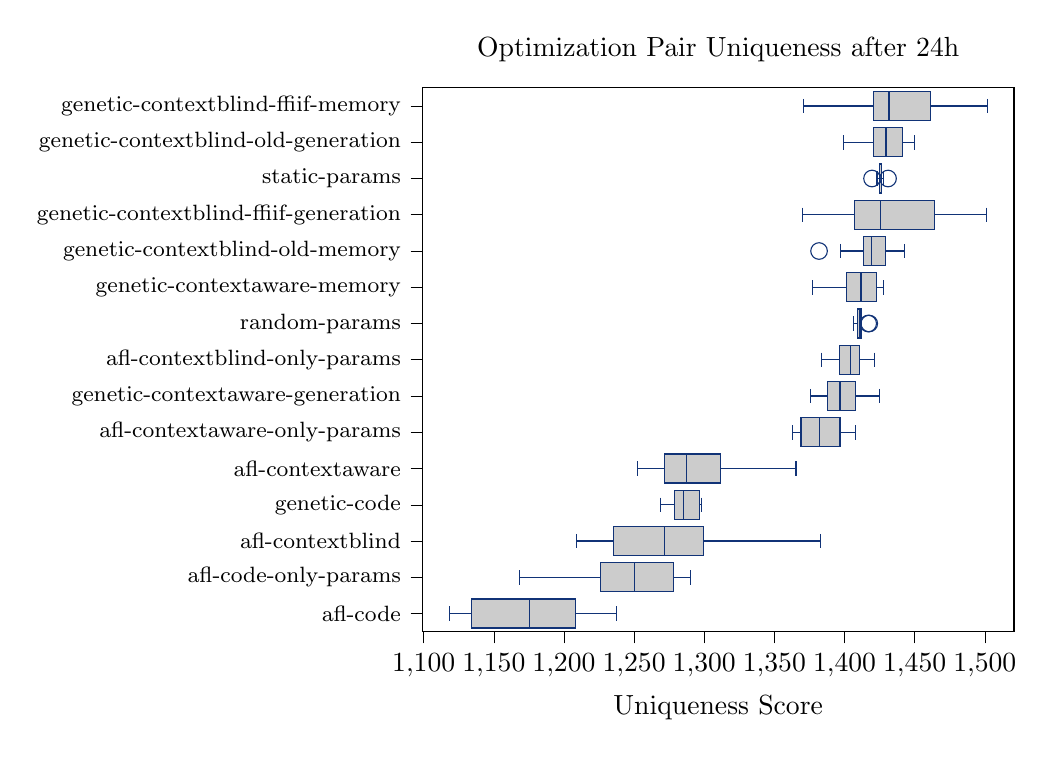
\begin{tikzpicture}

\definecolor{darkgray176}{RGB}{176,176,176}
\definecolor{lightgray204}{RGB}{204,204,204}
\definecolor{midnightblue1751119}{RGB}{17,51,119}

\begin{axis}[
tick align=outside,
tick pos=left,
title={Optimization Uniqueness Distribution (Final State)},
width=\linewidth,
x grid style={darkgray176},
xlabel={Uniqueness Score},
xmin=1099.10946643277, xmax=1520.79900348627,
xtick style={color=black},
y dir=reverse,
y grid style={darkgray176},
ymin=-0.5, ymax=14.5,
ytick style={color=black},
ytick={0,1,2,3,4,5,6,7,8,9,10,11,12,13,14},
yticklabels={
  genetic-contextblind-ffiif-memory,
  genetic-contextblind-old-generation,
  static-params,
  genetic-contextblind-ffiif-generation,
  genetic-contextblind-old-memory,
  genetic-contextaware-memory,
  random-params,
  afl-contextblind-only-params,
  genetic-contextaware-generation,
  afl-contextaware-only-params,
  afl-contextaware,
  genetic-code,
  afl-contextblind,
  afl-code-only-params,
  afl-code
}
]
\path [draw=midnightblue1751119, fill=lightgray204]
(axis cs:1420.65370430417,-0.4)
--(axis cs:1420.65370430417,0.4)
--(axis cs:1461.0904592425,0.4)
--(axis cs:1461.0904592425,-0.4)
--(axis cs:1420.65370430417,-0.4)
--cycle;
\addplot [midnightblue1751119]
table {%
1420.65370430417 0
1370.80028216035 0
};
\addplot [midnightblue1751119]
table {%
1461.0904592425 0
1501.63129725657 0
};
\addplot [midnightblue1751119]
table {%
1370.80028216035 -0.2
1370.80028216035 0.2
};
\addplot [midnightblue1751119]
table {%
1501.63129725657 -0.2
1501.63129725657 0.2
};
\path [draw=midnightblue1751119, fill=lightgray204]
(axis cs:1420.7585152318,0.6)
--(axis cs:1420.7585152318,1.4)
--(axis cs:1441.62081620477,1.4)
--(axis cs:1441.62081620477,0.6)
--(axis cs:1420.7585152318,0.6)
--cycle;
\addplot [midnightblue1751119]
table {%
1420.7585152318 1
1399.53500513717 1
};
\addplot [midnightblue1751119]
table {%
1441.62081620477 1
1449.76119113495 1
};
\addplot [midnightblue1751119]
table {%
1399.53500513717 0.8
1399.53500513717 1.2
};
\addplot [midnightblue1751119]
table {%
1449.76119113495 0.8
1449.76119113495 1.2
};
\path [draw=midnightblue1751119, fill=lightgray204]
(axis cs:1424.96472601644,1.6)
--(axis cs:1424.96472601644,2.4)
--(axis cs:1426.58133777807,2.4)
--(axis cs:1426.58133777807,1.6)
--(axis cs:1424.96472601644,1.6)
--cycle;
\addplot [midnightblue1751119]
table {%
1424.96472601644 2
1423.16290710207 2
};
\addplot [midnightblue1751119]
table {%
1426.58133777807 2
1427.4581410835 2
};
\addplot [midnightblue1751119]
table {%
1423.16290710207 1.8
1423.16290710207 2.2
};
\addplot [midnightblue1751119]
table {%
1427.4581410835 1.8
1427.4581410835 2.2
};
\addplot [black, mark=o, mark size=3, mark options={solid,fill opacity=0,draw=midnightblue1751119}, only marks]
table {%
1419.59590843234 2
1431.01212913747 2
};
\path [draw=midnightblue1751119, fill=lightgray204]
(axis cs:1407.12261289619,2.6)
--(axis cs:1407.12261289619,3.4)
--(axis cs:1463.93139298699,3.4)
--(axis cs:1463.93139298699,2.6)
--(axis cs:1407.12261289619,2.6)
--cycle;
\addplot [midnightblue1751119]
table {%
1407.12261289619 3
1369.9320181696 3
};
\addplot [midnightblue1751119]
table {%
1463.93139298699 3
1501.23108711934 3
};
\addplot [midnightblue1751119]
table {%
1369.9320181696 2.8
1369.9320181696 3.2
};
\addplot [midnightblue1751119]
table {%
1501.23108711934 2.8
1501.23108711934 3.2
};
\path [draw=midnightblue1751119, fill=lightgray204]
(axis cs:1413.80732375024,3.6)
--(axis cs:1413.80732375024,4.4)
--(axis cs:1428.90613047095,4.4)
--(axis cs:1428.90613047095,3.6)
--(axis cs:1413.80732375024,3.6)
--cycle;
\addplot [midnightblue1751119]
table {%
1413.80732375024 4
1396.80973258614 4
};
\addplot [midnightblue1751119]
table {%
1428.90613047095 4
1442.65570336829 4
};
\addplot [midnightblue1751119]
table {%
1396.80973258614 3.8
1396.80973258614 4.2
};
\addplot [midnightblue1751119]
table {%
1442.65570336829 3.8
1442.65570336829 4.2
};
\addplot [black, mark=o, mark size=3, mark options={solid,fill opacity=0,draw=midnightblue1751119}, only marks]
table {%
1381.8384508219 4
};
\path [draw=midnightblue1751119, fill=lightgray204]
(axis cs:1401.42802623561,4.6)
--(axis cs:1401.42802623561,5.4)
--(axis cs:1422.73818376056,5.4)
--(axis cs:1422.73818376056,4.6)
--(axis cs:1401.42802623561,4.6)
--cycle;
\addplot [midnightblue1751119]
table {%
1401.42802623561 5
1377.42275555384 5
};
\addplot [midnightblue1751119]
table {%
1422.73818376056 5
1427.84182304711 5
};
\addplot [midnightblue1751119]
table {%
1377.42275555384 4.8
1377.42275555384 5.2
};
\addplot [midnightblue1751119]
table {%
1427.84182304711 4.8
1427.84182304711 5.2
};
\path [draw=midnightblue1751119, fill=lightgray204]
(axis cs:1409.09661151059,5.6)
--(axis cs:1409.09661151059,6.4)
--(axis cs:1411.76718086367,6.4)
--(axis cs:1411.76718086367,5.6)
--(axis cs:1409.09661151059,5.6)
--cycle;
\addplot [midnightblue1751119]
table {%
1409.09661151059 6
1406.1400597094 6
};
\addplot [midnightblue1751119]
table {%
1411.76718086367 6
1411.77017154179 6
};
\addplot [midnightblue1751119]
table {%
1406.1400597094 5.8
1406.1400597094 6.2
};
\addplot [midnightblue1751119]
table {%
1411.77017154179 5.8
1411.77017154179 6.2
};
\addplot [black, mark=o, mark size=3, mark options={solid,fill opacity=0,draw=midnightblue1751119}, only marks]
table {%
1417.63253866532 6
1416.84771851669 6
};
\path [draw=midnightblue1751119, fill=lightgray204]
(axis cs:1396.42833766223,6.6)
--(axis cs:1396.42833766223,7.4)
--(axis cs:1410.89134932837,7.4)
--(axis cs:1410.89134932837,6.6)
--(axis cs:1396.42833766223,6.6)
--cycle;
\addplot [midnightblue1751119]
table {%
1396.42833766223 7
1383.36651440937 7
};
\addplot [midnightblue1751119]
table {%
1410.89134932837 7
1421.45836302164 7
};
\addplot [midnightblue1751119]
table {%
1383.36651440937 6.8
1383.36651440937 7.2
};
\addplot [midnightblue1751119]
table {%
1421.45836302164 6.8
1421.45836302164 7.2
};
\path [draw=midnightblue1751119, fill=lightgray204]
(axis cs:1387.90490299268,7.6)
--(axis cs:1387.90490299268,8.4)
--(axis cs:1407.7154734784,8.4)
--(axis cs:1407.7154734784,7.6)
--(axis cs:1387.90490299268,7.6)
--cycle;
\addplot [midnightblue1751119]
table {%
1387.90490299268 8
1375.71871425944 8
};
\addplot [midnightblue1751119]
table {%
1407.7154734784 8
1424.93063259519 8
};
\addplot [midnightblue1751119]
table {%
1375.71871425944 7.8
1375.71871425944 8.2
};
\addplot [midnightblue1751119]
table {%
1424.93063259519 7.8
1424.93063259519 8.2
};
\path [draw=midnightblue1751119, fill=lightgray204]
(axis cs:1368.92532025992,8.6)
--(axis cs:1368.92532025992,9.4)
--(axis cs:1396.76251404772,9.4)
--(axis cs:1396.76251404772,8.6)
--(axis cs:1368.92532025992,8.6)
--cycle;
\addplot [midnightblue1751119]
table {%
1368.92532025992 9
1362.84257487455 9
};
\addplot [midnightblue1751119]
table {%
1396.76251404772 9
1407.65763804731 9
};
\addplot [midnightblue1751119]
table {%
1362.84257487455 8.8
1362.84257487455 9.2
};
\addplot [midnightblue1751119]
table {%
1407.65763804731 8.8
1407.65763804731 9.2
};
\path [draw=midnightblue1751119, fill=lightgray204]
(axis cs:1271.79689068658,9.6)
--(axis cs:1271.79689068658,10.4)
--(axis cs:1311.36131435135,10.4)
--(axis cs:1311.36131435135,9.6)
--(axis cs:1271.79689068658,9.6)
--cycle;
\addplot [midnightblue1751119]
table {%
1271.79689068658 10
1252.42167474449 10
};
\addplot [midnightblue1751119]
table {%
1311.36131435135 10
1365.41748868479 10
};
\addplot [midnightblue1751119]
table {%
1252.42167474449 9.8
1252.42167474449 10.2
};
\addplot [midnightblue1751119]
table {%
1365.41748868479 9.8
1365.41748868479 10.2
};
\path [draw=midnightblue1751119, fill=lightgray204]
(axis cs:1278.80202215791,10.6)
--(axis cs:1278.80202215791,11.4)
--(axis cs:1296.37705431289,11.4)
--(axis cs:1296.37705431289,10.6)
--(axis cs:1278.80202215791,10.6)
--cycle;
\addplot [midnightblue1751119]
table {%
1278.80202215791 11
1268.68576163016 11
};
\addplot [midnightblue1751119]
table {%
1296.37705431289 11
1298.03043245592 11
};
\addplot [midnightblue1751119]
table {%
1268.68576163016 10.8
1268.68576163016 11.2
};
\addplot [midnightblue1751119]
table {%
1298.03043245592 10.8
1298.03043245592 11.2
};
\path [draw=midnightblue1751119, fill=lightgray204]
(axis cs:1235.3517960264,11.6)
--(axis cs:1235.3517960264,12.4)
--(axis cs:1299.30719106888,12.4)
--(axis cs:1299.30719106888,11.6)
--(axis cs:1235.3517960264,11.6)
--cycle;
\addplot [midnightblue1751119]
table {%
1235.3517960264 12
1208.6166726443 12
};
\addplot [midnightblue1751119]
table {%
1299.30719106888 12
1382.97070315399 12
};
\addplot [midnightblue1751119]
table {%
1208.6166726443 11.8
1208.6166726443 12.2
};
\addplot [midnightblue1751119]
table {%
1382.97070315399 11.8
1382.97070315399 12.2
};
\path [draw=midnightblue1751119, fill=lightgray204]
(axis cs:1225.88076229124,12.6)
--(axis cs:1225.88076229124,13.4)
--(axis cs:1277.97894766275,13.4)
--(axis cs:1277.97894766275,12.6)
--(axis cs:1225.88076229124,12.6)
--cycle;
\addplot [midnightblue1751119]
table {%
1225.88076229124 13
1168.51637752774 13
};
\addplot [midnightblue1751119]
table {%
1277.97894766275 13
1290.01713226872 13
};
\addplot [midnightblue1751119]
table {%
1168.51637752774 12.8
1168.51637752774 13.2
};
\addplot [midnightblue1751119]
table {%
1290.01713226872 12.8
1290.01713226872 13.2
};
\path [draw=midnightblue1751119, fill=lightgray204]
(axis cs:1134.09932967528,13.6)
--(axis cs:1134.09932967528,14.4)
--(axis cs:1207.97745942132,14.4)
--(axis cs:1207.97745942132,13.6)
--(axis cs:1134.09932967528,13.6)
--cycle;
\addplot [midnightblue1751119]
table {%
1134.09932967528 14
1118.27717266247 14
};
\addplot [midnightblue1751119]
table {%
1207.97745942132 14
1237.38163034107 14
};
\addplot [midnightblue1751119]
table {%
1118.27717266247 13.8
1118.27717266247 14.2
};
\addplot [midnightblue1751119]
table {%
1237.38163034107 13.8
1237.38163034107 14.2
};
\addplot [midnightblue1751119]
table {%
1431.69631402081 -0.4
1431.69631402081 0.4
};
\addplot [midnightblue1751119]
table {%
1429.59180750733 0.6
1429.59180750733 1.4
};
\addplot [midnightblue1751119]
table {%
1426.25127288117 1.6
1426.25127288117 2.4
};
\addplot [midnightblue1751119]
table {%
1425.56073140991 2.6
1425.56073140991 3.4
};
\addplot [midnightblue1751119]
table {%
1419.25888949408 3.6
1419.25888949408 4.4
};
\addplot [midnightblue1751119]
table {%
1411.71321082972 4.6
1411.71321082972 5.4
};
\addplot [midnightblue1751119]
table {%
1410.61947547669 5.6
1410.61947547669 6.4
};
\addplot [midnightblue1751119]
table {%
1404.38663605407 6.6
1404.38663605407 7.4
};
\addplot [midnightblue1751119]
table {%
1396.73141369904 7.6
1396.73141369904 8.4
};
\addplot [midnightblue1751119]
table {%
1382.05754898943 8.6
1382.05754898943 9.4
};
\addplot [midnightblue1751119]
table {%
1287.31395316225 9.6
1287.31395316225 10.4
};
\addplot [midnightblue1751119]
table {%
1285.45923206501 10.6
1285.45923206501 11.4
};
\addplot [midnightblue1751119]
table {%
1271.53462794507 11.6
1271.53462794507 12.4
};
\addplot [midnightblue1751119]
table {%
1250.23660234985 12.6
1250.23660234985 13.4
};
\addplot [midnightblue1751119]
table {%
1175.42564949101 13.6
1175.42564949101 14.4
};
\end{axis}

\end{tikzpicture}
%
    \endgroup
    \caption{Uniqueness scores of different configurations (and variants) based on triggered rare optimizations.
    \label{fig:rare-opts}
    See \cref{ss:eval-rare-opts} for details.}
\end{figure}

\begin{figure}[t]
    \centering
    \begingroup
    \pgfplotsset{
        every axis/.append style={
            yticklabel style={font=\propernamedecl\footnotesize},
            execute at begin axis={
                \pgfplotsset{title={Optimization Pair Uniqueness after 24h},
                    width=0.75\textwidth,
                    height=0.7\linewidth}
            },
        },
    }
    % This file was created with matplot2tikz v0.4.0.
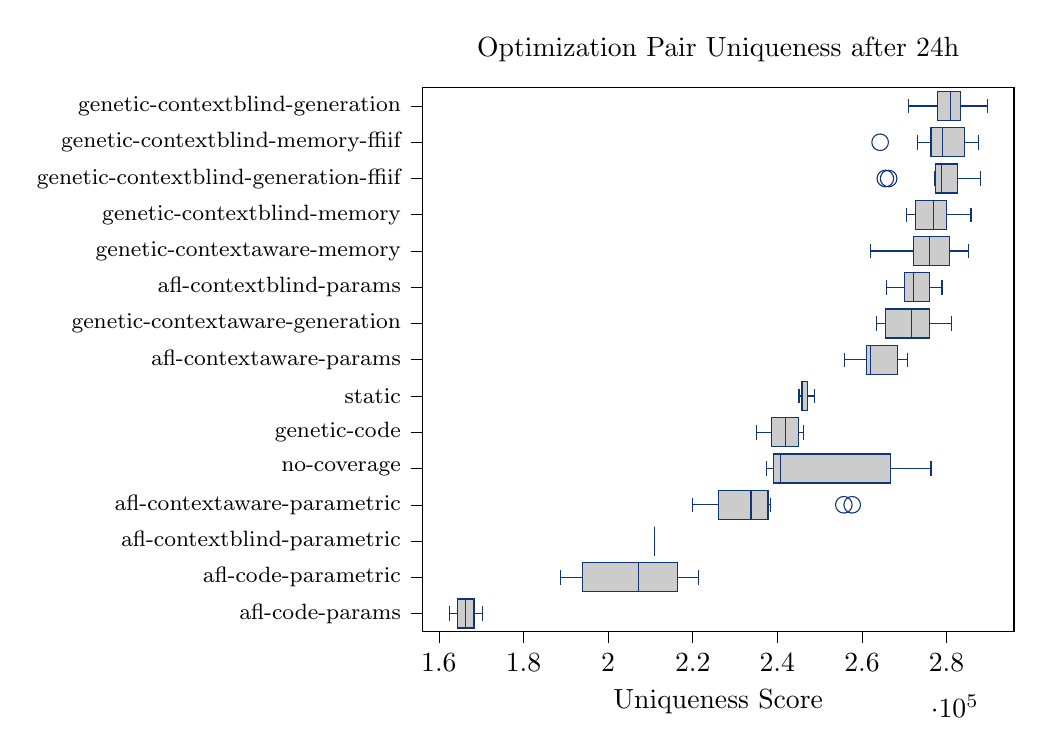
\begin{tikzpicture}

\definecolor{darkgray176}{RGB}{176,176,176}
\definecolor{lightgray204}{RGB}{204,204,204}
\definecolor{midnightblue1751119}{RGB}{17,51,119}

\begin{axis}[
tick align=outside,
tick pos=left,
title={OptimizationPair Uniqueness at Final Time Step},
width=\linewidth,
x grid style={darkgray176},
xlabel={Uniqueness Score},
xmin=156120.909333459, xmax=295943.441329031,
xtick style={color=black},
y dir=reverse,
y grid style={darkgray176},
ymin=-0.5, ymax=14.5,
ytick style={color=black},
ytick={0,1,2,3,4,5,6,7,8,9,10,11,12,13,14},
yticklabels={
  genetic-contextblind-generation,
  genetic-contextblind-memory-ffiif,
  genetic-contextblind-generation-ffiif,
  genetic-contextblind-memory,
  genetic-contextaware-memory,
  afl-contextblind-params,
  genetic-contextaware-generation,
  afl-contextaware-params,
  static,
  genetic-code,
  no-coverage,
  afl-contextaware-parametric,
  afl-contextblind-parametric,
  afl-code-parametric,
  afl-code-params
}
]
\path [draw=midnightblue1751119, fill=lightgray204]
(axis cs:277953.440212219,-0.4)
--(axis cs:277953.440212219,0.4)
--(axis cs:283315.846064258,0.4)
--(axis cs:283315.846064258,-0.4)
--(axis cs:277953.440212219,-0.4)
--cycle;
\addplot [midnightblue1751119]
table {%
277953.440212219 0
271030.361656792 0
};
\addplot [midnightblue1751119]
table {%
283315.846064258 0
289587.871692869 0
};
\addplot [midnightblue1751119]
table {%
271030.361656792 -0.2
271030.361656792 0.2
};
\addplot [midnightblue1751119]
table {%
289587.871692869 -0.2
289587.871692869 0.2
};
\path [draw=midnightblue1751119, fill=lightgray204]
(axis cs:276321.450477075,0.6)
--(axis cs:276321.450477075,1.4)
--(axis cs:284223.966778089,1.4)
--(axis cs:284223.966778089,0.6)
--(axis cs:276321.450477075,0.6)
--cycle;
\addplot [midnightblue1751119]
table {%
276321.450477075 1
273228.864873659 1
};
\addplot [midnightblue1751119]
table {%
284223.966778089 1
287500.8122168 1
};
\addplot [midnightblue1751119]
table {%
273228.864873659 0.8
273228.864873659 1.2
};
\addplot [midnightblue1751119]
table {%
287500.8122168 0.8
287500.8122168 1.2
};
\addplot [black, mark=o, mark size=3, mark options={solid,fill opacity=0,draw=midnightblue1751119}, only marks]
table {%
264299.494248465 1
};
\path [draw=midnightblue1751119, fill=lightgray204]
(axis cs:277319.142230507,1.6)
--(axis cs:277319.142230507,2.4)
--(axis cs:282626.637877005,2.4)
--(axis cs:282626.637877005,1.6)
--(axis cs:277319.142230507,1.6)
--cycle;
\addplot [midnightblue1751119]
table {%
277319.142230507 2
277179.393731311 2
};
\addplot [midnightblue1751119]
table {%
282626.637877005 2
288081.007370516 2
};
\addplot [midnightblue1751119]
table {%
277179.393731311 1.8
277179.393731311 2.2
};
\addplot [midnightblue1751119]
table {%
288081.007370516 1.8
288081.007370516 2.2
};
\addplot [black, mark=o, mark size=3, mark options={solid,fill opacity=0,draw=midnightblue1751119}, only marks]
table {%
266312.410583593 2
265533.361534734 2
};
\path [draw=midnightblue1751119, fill=lightgray204]
(axis cs:272745.983909547,2.6)
--(axis cs:272745.983909547,3.4)
--(axis cs:279910.873919318,3.4)
--(axis cs:279910.873919318,2.6)
--(axis cs:272745.983909547,2.6)
--cycle;
\addplot [midnightblue1751119]
table {%
272745.983909547 3
270428.785759479 3
};
\addplot [midnightblue1751119]
table {%
279910.873919318 3
285789.991942737 3
};
\addplot [midnightblue1751119]
table {%
270428.785759479 2.8
270428.785759479 3.2
};
\addplot [midnightblue1751119]
table {%
285789.991942737 2.8
285789.991942737 3.2
};
\path [draw=midnightblue1751119, fill=lightgray204]
(axis cs:272242.369144191,3.6)
--(axis cs:272242.369144191,4.4)
--(axis cs:280719.896229137,4.4)
--(axis cs:280719.896229137,3.6)
--(axis cs:272242.369144191,3.6)
--cycle;
\addplot [midnightblue1751119]
table {%
272242.369144191 4
261953.664031869 4
};
\addplot [midnightblue1751119]
table {%
280719.896229137 4
285093.423611437 4
};
\addplot [midnightblue1751119]
table {%
261953.664031869 3.8
261953.664031869 4.2
};
\addplot [midnightblue1751119]
table {%
285093.423611437 3.8
285093.423611437 4.2
};
\path [draw=midnightblue1751119, fill=lightgray204]
(axis cs:270081.277302514,4.6)
--(axis cs:270081.277302514,5.4)
--(axis cs:275884.144553685,5.4)
--(axis cs:275884.144553685,4.6)
--(axis cs:270081.277302514,4.6)
--cycle;
\addplot [midnightblue1751119]
table {%
270081.277302514 5
265717.47506831 5
};
\addplot [midnightblue1751119]
table {%
275884.144553685 5
278912.194976947 5
};
\addplot [midnightblue1751119]
table {%
265717.47506831 4.8
265717.47506831 5.2
};
\addplot [midnightblue1751119]
table {%
278912.194976947 4.8
278912.194976947 5.2
};
\path [draw=midnightblue1751119, fill=lightgray204]
(axis cs:265530.544856777,5.6)
--(axis cs:265530.544856777,6.4)
--(axis cs:275921.235648894,6.4)
--(axis cs:275921.235648894,5.6)
--(axis cs:265530.544856777,5.6)
--cycle;
\addplot [midnightblue1751119]
table {%
265530.544856777 6
263426.390826741 6
};
\addplot [midnightblue1751119]
table {%
275921.235648894 6
281180.182736596 6
};
\addplot [midnightblue1751119]
table {%
263426.390826741 5.8
263426.390826741 6.2
};
\addplot [midnightblue1751119]
table {%
281180.182736596 5.8
281180.182736596 6.2
};
\path [draw=midnightblue1751119, fill=lightgray204]
(axis cs:260987.75900005,6.6)
--(axis cs:260987.75900005,7.4)
--(axis cs:268397.679125152,7.4)
--(axis cs:268397.679125152,6.6)
--(axis cs:260987.75900005,6.6)
--cycle;
\addplot [midnightblue1751119]
table {%
260987.75900005 7
255842.604688313 7
};
\addplot [midnightblue1751119]
table {%
268397.679125152 7
270686.664141726 7
};
\addplot [midnightblue1751119]
table {%
255842.604688313 6.8
255842.604688313 7.2
};
\addplot [midnightblue1751119]
table {%
270686.664141726 6.8
270686.664141726 7.2
};
\path [draw=midnightblue1751119, fill=lightgray204]
(axis cs:245710.451474509,7.6)
--(axis cs:245710.451474509,8.4)
--(axis cs:247064.132193546,8.4)
--(axis cs:247064.132193546,7.6)
--(axis cs:245710.451474509,7.6)
--cycle;
\addplot [midnightblue1751119]
table {%
245710.451474509 8
245115.571542708 8
};
\addplot [midnightblue1751119]
table {%
247064.132193546 8
248703.81213221 8
};
\addplot [midnightblue1751119]
table {%
245115.571542708 7.8
245115.571542708 8.2
};
\addplot [midnightblue1751119]
table {%
248703.81213221 7.8
248703.81213221 8.2
};
\path [draw=midnightblue1751119, fill=lightgray204]
(axis cs:238623.700293406,8.6)
--(axis cs:238623.700293406,9.4)
--(axis cs:245080.272090991,9.4)
--(axis cs:245080.272090991,8.6)
--(axis cs:238623.700293406,8.6)
--cycle;
\addplot [midnightblue1751119]
table {%
238623.700293406 9
235074.155260022 9
};
\addplot [midnightblue1751119]
table {%
245080.272090991 9
246090.619086918 9
};
\addplot [midnightblue1751119]
table {%
235074.155260022 8.8
235074.155260022 9.2
};
\addplot [midnightblue1751119]
table {%
246090.619086918 8.8
246090.619086918 9.2
};
\path [draw=midnightblue1751119, fill=lightgray204]
(axis cs:239009.293847989,9.6)
--(axis cs:239009.293847989,10.4)
--(axis cs:266811.79701274,10.4)
--(axis cs:266811.79701274,9.6)
--(axis cs:239009.293847989,9.6)
--cycle;
\addplot [midnightblue1751119]
table {%
239009.293847989 10
237428.122246795 10
};
\addplot [midnightblue1751119]
table {%
266811.79701274 10
276330.540146626 10
};
\addplot [midnightblue1751119]
table {%
237428.122246795 9.8
237428.122246795 10.2
};
\addplot [midnightblue1751119]
table {%
276330.540146626 9.8
276330.540146626 10.2
};
\path [draw=midnightblue1751119, fill=lightgray204]
(axis cs:226197.261310072,10.6)
--(axis cs:226197.261310072,11.4)
--(axis cs:237803.38032637,11.4)
--(axis cs:237803.38032637,10.6)
--(axis cs:226197.261310072,10.6)
--cycle;
\addplot [midnightblue1751119]
table {%
226197.261310072 11
219846.467137529 11
};
\addplot [midnightblue1751119]
table {%
237803.38032637 11
238324.704512253 11
};
\addplot [midnightblue1751119]
table {%
219846.467137529 10.8
219846.467137529 11.2
};
\addplot [midnightblue1751119]
table {%
238324.704512253 10.8
238324.704512253 11.2
};
\addplot [black, mark=o, mark size=3, mark options={solid,fill opacity=0,draw=midnightblue1751119}, only marks]
table {%
255720.264480067 11
257695.031778287 11
};
\path [draw=midnightblue1751119, fill=lightgray204]
(axis cs:211033.329712607,11.6)
--(axis cs:211033.329712607,12.4)
--(axis cs:211033.329712607,12.4)
--(axis cs:211033.329712607,11.6)
--(axis cs:211033.329712607,11.6)
--cycle;
\addplot [midnightblue1751119]
table {%
211033.329712607 12
211033.329712607 12
};
\addplot [midnightblue1751119]
table {%
211033.329712607 12
211033.329712607 12
};
\addplot [midnightblue1751119]
table {%
211033.329712607 11.8
211033.329712607 12.2
};
\addplot [midnightblue1751119]
table {%
211033.329712607 11.8
211033.329712607 12.2
};
\path [draw=midnightblue1751119, fill=lightgray204]
(axis cs:193986.829759283,12.6)
--(axis cs:193986.829759283,13.4)
--(axis cs:216309.391668908,13.4)
--(axis cs:216309.391668908,12.6)
--(axis cs:193986.829759283,12.6)
--cycle;
\addplot [midnightblue1751119]
table {%
193986.829759283 13
188729.334355677 13
};
\addplot [midnightblue1751119]
table {%
216309.391668908 13
221452.703553717 13
};
\addplot [midnightblue1751119]
table {%
188729.334355677 12.8
188729.334355677 13.2
};
\addplot [midnightblue1751119]
table {%
221452.703553717 12.8
221452.703553717 13.2
};
\path [draw=midnightblue1751119, fill=lightgray204]
(axis cs:164420.581305993,13.6)
--(axis cs:164420.581305993,14.4)
--(axis cs:168308.785978736,14.4)
--(axis cs:168308.785978736,13.6)
--(axis cs:164420.581305993,13.6)
--cycle;
\addplot [midnightblue1751119]
table {%
164420.581305993 14
162476.478969621 14
};
\addplot [midnightblue1751119]
table {%
168308.785978736 14
170252.888315108 14
};
\addplot [midnightblue1751119]
table {%
162476.478969621 13.8
162476.478969621 14.2
};
\addplot [midnightblue1751119]
table {%
170252.888315108 13.8
170252.888315108 14.2
};
\addplot [midnightblue1751119]
table {%
280993.164952848 -0.4
280993.164952848 0.4
};
\addplot [midnightblue1751119]
table {%
279147.755892618 0.6
279147.755892618 1.4
};
\addplot [midnightblue1751119]
table {%
278738.741742052 1.6
278738.741742052 2.4
};
\addplot [midnightblue1751119]
table {%
276873.777026243 2.6
276873.777026243 3.4
};
\addplot [midnightblue1751119]
table {%
275895.950865476 3.6
275895.950865476 4.4
};
\addplot [midnightblue1751119]
table {%
272250.194229867 4.6
272250.194229867 5.4
};
\addplot [midnightblue1751119]
table {%
271706.921457256 5.6
271706.921457256 6.4
};
\addplot [midnightblue1751119]
table {%
262080.771506874 6.6
262080.771506874 7.4
};
\addplot [midnightblue1751119]
table {%
246010.571791481 7.6
246010.571791481 8.4
};
\addplot [midnightblue1751119]
table {%
241953.518655476 8.6
241953.518655476 9.4
};
\addplot [midnightblue1751119]
table {%
240854.54972975 9.6
240854.54972975 10.4
};
\addplot [midnightblue1751119]
table {%
233767.109931736 10.6
233767.109931736 11.4
};
\addplot [midnightblue1751119]
table {%
211033.329712607 11.6
211033.329712607 12.4
};
\addplot [midnightblue1751119]
table {%
207151.024234722 12.6
207151.024234722 13.4
};
\addplot [midnightblue1751119]
table {%
166364.683642365 13.6
166364.683642365 14.4
};
\end{axis}

\end{tikzpicture}
%
    \endgroup
    \caption{Uniqueness scores of different configurations (and variants) based on triggered rare optimization pairs.
    \label{fig:rare-pairs}
    See \cref{ss:eval-rare-opts} for details.}
\end{figure}


We evaluated both the rareness of single optimizations and the rareness of optimization pairs.
In the following text, we use \emph{feature} to mean either optimizations or optimization pairs.

We define the \enquote{rareness} $R(f)$ of a particular feature $f \in F$ as
\[ R(f) = \log\left( \frac{\sum_{f_j \in F}{\mathrm{count}(f_j)}}{\mathrm{count}(f)} \right) \]
where $\mathrm{count}(f)$ is the number of occurrences of $f$ across \emph{all} experiments.
That is, the less often a feature occurred in \emph{any} experiment, the rarer it is.
We only consider features that occurred at least once overall.
The logarithm scales down extremely common features, such as the \propername{CanonicalReplacement} optimization.
We found that due to the very high counts of these features, they would disproportionately contribute to an experiment's overall score, despite being so common.

Based on this definition we calculate a score for each run in a configuration that rates how many rare optimizations or optimization pairs the configuration triggered.
The score for a run is simply the sum of all individual feature scores in that run.
The boxplots in \cref{fig:rare-opts,fig:rare-pairs} illustrate statistics based on the rareness scores of the runs in a configuration.
The boxplot in \cref{fig:rare-opts} is based on optimization rareness scores and the boxplot in \cref{fig:rare-pairs} is based on optimization-pair rareness scores.
Note that the scores for optimizations and optimization pairs are not directly comparable.
